%!TEX options = --shell-escape


\documentclass[bachelor]{thesis-uestc}

\title{全路网智能路径规划}
\author{董林森}
\advisor{郭宏亮\chinesespace 副教授}
\school{自动化工程学院}
\major{测控技术与仪器}
\studentid{2014070906006}

\begin{document}

% \makecover

% this is a thesis template with mutiple files: the chapters and the misc in standalone mode
% to avoid too many files in current folder, template add extra direcotry: chapter and misc
% please do not change the sequence of each one except the chapters themselves.
% by FengYouzheng.

% abstract
\documentclass{standalone}
% preamble: usepackage, etc.
\begin{document}
	
\begin{chineseabstract}

在一个交通网络中,给定起点和终点,给出一条最优路径已经作为一种算法,广泛的应用到了实际生活中。这类算法一般被称为路径规划算法,或者最短路径算法。随着交通网络的复杂,多种交通工具的发展,传统的基于静态地图的路径规划算法已无法适应日渐复杂的环境,如何实现出更加强大和灵活的路径规划算法已经成为各国学者的一个研究重点。

随着人工智能和机器学习的快速发展,强化学习,作为一个该领域的一个重要分支,展现它在很多领域的应用潜力,比如围棋等。作为一个决策和控制的框架,强化学习同样可以被应用在路径规划系统。在我们的工作中,我们使用强化学习解决路径规划问题,并且解决了多个不同的路径规划场景问题,特别是解决了一些传统的基于搜索的路径规划算法,比如 $A^{*}$,$Dijkstra$ 等不能解决的场景。

论文分为五个部分,在第一章,我们给出了路径规划问题的基本数学形式,同时我们给出了几种基于基本路径规划问题的变形,例如带有额外转弯惩罚的路径规划问题,带有行驶长度限制的电动车路径规划问题,以及动态地图环境下的路径规划。这些特殊的场景是传统的最短路径算法所难以解决的,我们将通过强化学习的方法很好的解决这些场景;在第二章,我们先给出传统的基于搜索的路径规划算法,例如 $A^*,Dijkstra$等,并给出为了解决以上特殊场景而做出的一些改进算法。同时我们试着简单分析这类方法的缺点,例如不够灵活,无法应对复杂动态环境或更复杂的用户需求等;在第三章,我们给出强化学习的基本概念和相关方法,包括了强化学习的基于智能体建模的方法和基于马尔科夫决策过程的控制结构。以及强化学习中的基本概念,如价值函数,策略函数等,最后着重介绍为了解决路径规划问题使用的基于值函数的方法;在第四章,我们将介绍我们的方法,首先将路径规划问题表述为一个标准的马尔科夫决策过程,然后针对不同的环境,我们设计了基于 $Q-learning$ 的强化学习算法。在第五章,我们给出了具体的代码实现方法和实验结果;最后给出全文的总结和未来的研究方向。

\chinesekeyword{强化学习,路径规划}
\end{chineseabstract}

\end{document}
\documentclass{standalone}
% preamble: usepackage, etc.
\begin{document}

\begin{englishabstract}
    With the development of Artificial Intelligence and Machine Learning, Reinforcement Learning, as an important method in this field, have showed its great potential in field like Go. As a decision-making and control schema, reinforcement learning also can be applied in route planning system, which is a widely used system in navigation system … In our work, we applied reinforcement learning to route planning problem and solved various scenarios, especially for the scenario that traditional search-based route planning algorithms like Dijkstra and  search can’t solve. 
    
    The content of the dissertation is divided into three parts, firstly, we give the mathematical formulation of route planning problem, and adapted it into Markov Decision Process. Then we adapted it to different scenarios with modification of original formulation. At last, we compared our reinforcement learning based method with search based method which regard as the baseline under different experiments.
    
    Our main contributions are 1) firstly applied reinforcement learning into online-routing service 2) showed the flexibility of reinforcement learning with different metric function, scenarios and even dynamics environment.

	\englishkeyword{route planning, routing service, reinforcement learning, online learning}
\end{englishabstract}

\end{document}

% table of contents
\thesistableofcontents

% thesis contents
\documentclass{standalone}
% preamble: usepackage, etc.
\begin{document}

\thesischapterexordium

\section{研究工作的背景与意义}
随着城市交通网络的发展和交通工具的进步,针对路径规划问题设计的各种系统和算法逐渐在现实生活中被广泛的应用,比如在日常驾驶出行或乘坐公共交通等情景中,人们越来越频繁的使用这一功能。同时随着交通网络复杂度提高,规模增大,多种交通工具的出现以及城市堵车给城市交通网络带来的随机性和动态性,这给传统的路径规划问题带来了全面的挑战。同样,随着自动驾驶技术的发展,路径规划问题作为自动驾驶的导航模块中重要的部分同样扮演者不可或缺的角色。因此如何更好的设计出更强大,更具灵活性的,更高效的路径规划算法具有重要的发展意义,而这也成为了当前各国学者的研究热点之一。

% \footnote{脚注序号“\ding{172},……,\ding{180}”的字体是“正文”,不是“上标”,序号与脚注内容文字之间空1个半角字符,脚注的段落格式为:单倍行距,段前空0磅,段后空0磅,悬挂缩进1.5字符;中文用宋体,字号为小五号,英文和数字用Times New Roman字体,字号为9磅;中英文混排时,所有标点符号(例如逗号“,”、括号“()”等)一律使用中文输入状态下的标点符号,但小数点采用英文状态下的样式“.”。}

\section{路径规划问题的国内外研究历史与现状}
路径规划问题,根据问题形式不同,分为完备的路径规划和基于采样,或称为概率完备的路径规划。基于采样的方法是为了解决三维空间高复杂度情况下的路径规划问题,包括了 PRM, RRT等一系列方法。在本文中,我们重点讨论基于完备的路径规划,完备意为给定起点和终点,,我们拥有交通网络环境的全局信息。基于完备地图的路径规划最早被转换为图论中的最短路径问题,最短路径问题根据图的类型不同,首先分为无向图上的最短路径、有向图上的最短路径、单源最短路,多源最短路等等。Edsger W. Dijkstra 最早于1956年,提出了著名的 $Dijkstra$ 算法,给出了单源最短路算法,随后包括 $Bellman-Ford$, $A^* search$, $Floyd-Warshall$ $Johnson's algorithm$, $Viterbi algorithm$等被相继提出,在一定程度上都降低了最短路算法的时空复杂度。\par
但随着交通环境复杂度的增加(大陆级别的地图范围)和用户需求的增加(例如需要考虑多种交通工具的组合,倾向选择公共交通方式,选择非收费路段等),先前提出的基于静态网络和单一的度量方法都已经无法适应。因此各国学者和研究机构,例如Microsoft,Karlsruhe Institute of Technology等针对不同的场景,提出了改进的算法。

\section{本文的主要贡献与创新}
我们的主要贡献包括:1)首次将端到端的强化学习应用到了路径规划算法,并证明了其可用性。2)使用强化学习解决了传统算法难以解决的某些路径规划场景。

\section{本论文的结构安排}
本文的章节结构安排如下:\par
论文分为五个部分,在第一章,我们给出了路径规划问题的基本数学形式,同时我们给出了几种基于基本路径规划问题的变形,例如带有额外转弯惩罚的路径规划问题,带有行驶长度限制的电动车路径规划问题,以及动态地图环境下的路径规划。这些特殊的场景是传统的最短路径算法所难以解决的,我们将通过强化学习的方法很好的解决这些场景;在第二章,我们先给出传统的基于搜索的路径规划算法,例如 $A^{*}$,$Dijkstra$ 等,并给出为了解决以上特殊场景而做出的一些改进算法。同时我们试着简单分析这类方法的缺点,例如不够灵活,无法应对复杂动态环境或更复杂的用户需求等;在第三章,我们给出强化学习的基本概念和相关方法,包括了强化学习的基于智能体建模的方法和基于马尔科夫决策过程的控制结构。以及强化学习中的基本概念,如价值函数,策略函数等,最后着重介绍为了解决路径规划问题使用的基于值函数的方法;在第四章,我们将介绍我们的方法,首先将路径规划问题表述为一个标准的马尔科夫决策过程,然后针对不同的环境,我们设计了基于 $Q-learning$ 的强化学习算法。在第五章,我们给出了具体的代码实现方法和实验结果;最后给出全文的总结和未来的研究方向。

\end{document}
\documentclass{standalone}
% preamble: usepackage, etc.
\usepackage{tikz}
\usepackage{amsmath}

\begin{document}

\chapter{路径规划问题}
在这一章,我们引入路径规划问题,给出其严格的数学定义。然后介绍随着现实世界的变化,路径规划问题所出现的新的形式和挑战,然后给出其数学形式。通过这一章,我们将详细阐述我们的工作所解决的问题,以及有利于相关强化学习算法的设计和实验。
\section{路径规划问题的数学形式}
路径规划问题,如绪论1.2节所述,根据问题建模形式,其算法分为基于图的搜索算法和基于采样的规划方法。在本文中,我们使用基于图的搜索算法,然后给出其相应的数学形式。\par
令 $v\in \{1,2,3...n\}$表示图中的某个顶点,假设有$n$个顶点。令$e_i,j$表示图中的一条从点$i$到点$j$的一条边,假设共有$m$条边。令$V$ 表示图中节点的集合,令$E=\{e_i,j)| i,j \in V \}$表示图中边的集合。
令$f:E \to \mathbb{R}$ 表示为一个将图中的任意一条边映射到某一实数集上的函数,在静态的最短路径问题中,该函数一般等价于路径长度,但在本文中,为了使模型和算法应用于多种场景中,我们将其定义为抽象的损失函数,即通过某条边的损失,以使得定义能够适应于复杂的路径规划场景。$f$函数的输入包括但不限于某条边,在不同问题中,可能会有额外的输入信息以计算该函数值,例如在带有转弯额外惩罚的场景中,车辆是否转弯也作为函数的输入以计算损失值。则由以上定义可得一个有向图定义为$G=(V, E, f)$,其包含一个点集$V$,一个边集$E$和一个损失函数$f$。

我们定义$P=\{v_1, v_2,...,v_k\}$为图中的一条路径,路径的长度或总损失定义为$L(P) = \sum_{i=1}^{j-1} f(e_{v_i,v_{i+1}})$。基于以上定义,最短路径规划问题可以被定义为:在图$G$中,给定某一起始点$v_s$和终止点$v_t$,找到某一条路径$P_{optimal}$使得$L(P_{optimal})$最小,公式定义如下:
\begin{center}
\begin{equation}
P_{optimal} = argmin_{P}(L(P))
\end{equation}
\end{center}

where $v_s$ is the start node of $P$, $v_t$ is the end node of $P$.\par
一个简单的实例如图2-1所示,标注蓝色的边表示了从节点 A 到节点 F 的最短路径。
\begin{figure}[h]
	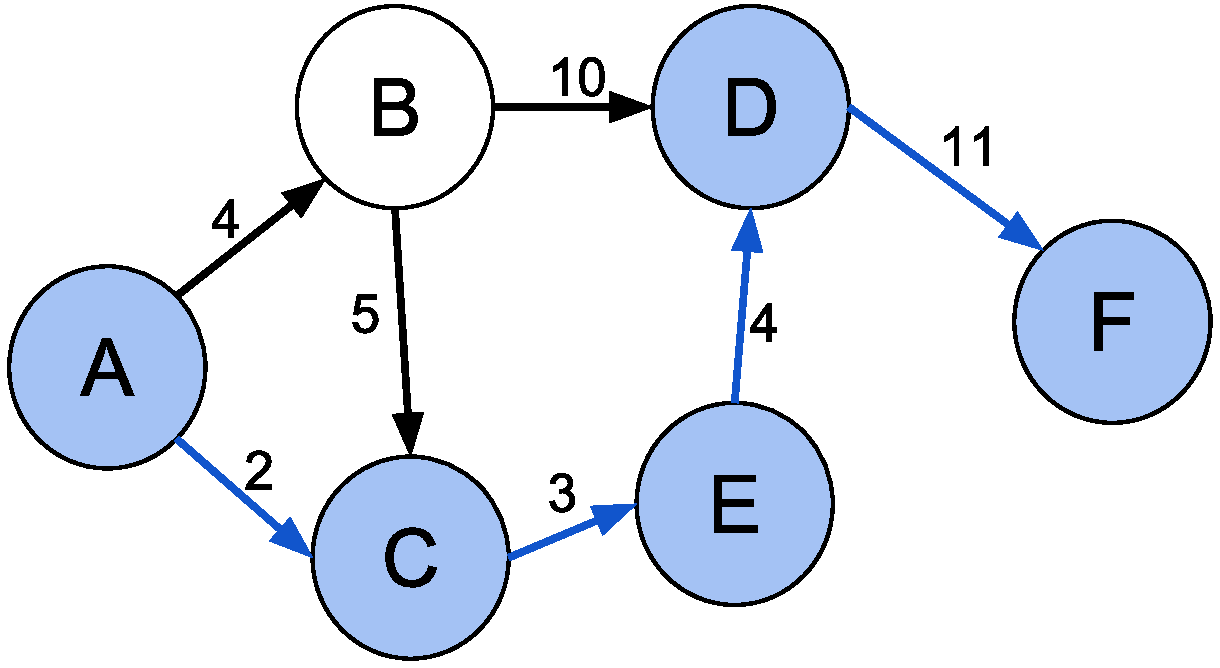
\includegraphics[width=12.0cm]{pic/2-1.pdf}
	\caption{最短路径求解示例}
	\label{2-1}
\end{figure}

\section{不同场景及其数学形式}
在这一章节,我们将介绍基于2.1章节基本最短路径问题形式的几个特殊场景,这些场景是由于随着现代交通网路的发展和复杂化,以及交通工具的扩展而出现的一些不同于传统形式的特殊场景。这些场景的出现使得我们需要对原有的问题形式进行一定的修改和重新定义,以方便我们进行相应算法的设计和实现。在本章节中将要介绍的场景也是我们将要使用强化学习进行应用和解决的场景。通过给出其数学形式上的严格定义,有助于我们在随后进行基于马尔科夫决策过程的建模和强化学习算法的设计。

\subsection{场景1:简单网格地图}
第一个场景为简单网格地图场景,设计该场景的原因在于,我们将通过这一简单的场景验证强化学习模型在路径规划问题上的可用性。在该场景中,我们通过一个二维网格表示地图,在任意一个点,在不越过地图界限的情况下,车辆可以向上下左右四个方向移动,如图2-2所示。令 $N$ 表示图的行数, $M$表示图的列数,左下角点的坐标为$(0,0)$,右上角的坐标为$(N-1, M-1)$。在图中,w我们定义$S$ 为起点,$E$为目标点,某一时刻,车辆所处的位置由图中的$car$ 点表示。车辆在移动过程中,其每次移动距离为一个格子,边上的损失函数 定义为:
\begin{center}
    \begin{equation}
    f(e_{v_i,v_{i+1}}) = C, C\in\mathbb{R}, C\ge0 \text{且$C$为常数}
\end{equation}
\end{center}

\begin{figure}[H]
\begin{center}
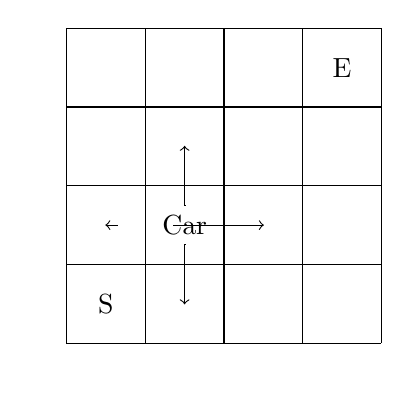
\begin{tikzpicture}[every node/.style={minimum size=1cm-\pgflinewidth, outer sep=0pt}, arrow/.style={thick}]
    \draw[step=1cm,color=black] (-2,-2) grid (2,2); 
    \node[](start) at (-1.5, -1.5) {S};
    \node[](end) at (1.5, 1.5) {E};
    \node[](car) at (-0.5, -0.5) {Car};
    
    \node[](car_up_center) at (0.0, -0.25) {};    
    \node[](car_up) at (-0.5, 1.0) {};
    
    \node[](car_down_center) at (0.0, -0.75) {};
    \node[](car_down) at (-0.5, -2.0){};

    \node[](car_left_center) at (-1.35, -0.5) {};
    \node[](car_left) at (-2.0, -0.5){};

    \node[](car_right_center) at (-0.65, -0.5) {};
    \node[](car_right) at (1.0, -0.5){};
    
    % \node[](charge site) at (-0.5, 1.5) {$t_{1}$};
    % \node[](charge site) at (1.5, -0.5) {$t_{2}$};
    \draw[->, to path={-| (\tikztotarget)}]
 	( car_up_center) edge (car_up)  (car_down_center) edge (car_down) ;
     \draw[<-, to path={-| (\tikztotarget)}]
 	(car_left) edge (car_left_center) (car_right) edge (car_right_center);
\end{tikzpicture}
\caption{场景1:简单网格地图}
\end{center}
\label{2-2}
\end{figure}

\subsection{场景2:带有转弯惩罚的场景}
在现实交通网络中,对最短路径计算结果具有重要影响的因素之一为转弯方向的选择,例如在图2-2实例中,同时存在多条从起点到终点的最短路径,但在实际交通网络中,例如中国等靠右行驶的国家中,左转往往比直行和右转具有更长的时间消耗。因此在两条最短路径行驶长度完全相同的情况下,较少左转的路径往往实际消耗的时间更少。
因此我们通过加入额外的转弯惩罚设计了场景2,在该场景中,在任意一条边上的移动损失函数定义为
\begin{center}
\begin{equation}
f(e_{v_i,v_{i+1}}) = \begin{cases}
C + A &\mbox{if car turn left or turn around}\\
C &\mbox{else}
\end{cases}
\end{equation}
\mbox{其中 }
$A \in\mathbb{R}, C\ge0$
\mbox{ 为常数,表示转弯的额外惩罚}
\end{center}

\subsection{场景3:带有行驶路径限制和充电桩的场景}
随着电动汽车的普及和推广,基于电动车的路径规划也作为某一特定问题被各国学者进行研究。该场景的特殊性在于,电动车普遍行驶距离较短,在进行单次路径规划中,我们在求解最短路径的同时,需要保证其在任意行驶过程中保持电量大于零,如果电量过低,需要到就近的充电桩进行充电后再行驶。
这给原始的简单网格地图的场景带来了如下变化:首先,地图中增加多个充电桩的位置,充电桩的集合被定义为 $T = \{t_{1}, t_{2}...,t_{k}\}, t_i \in V$;
同时对车辆,除去其当前位置,我们需要引入$\mathrm{power}\in[0, MAXPOWER]$表示车辆当前剩余电量。其中 $MAXPOWER\ge0$,表示车辆电量的最大值。修改后的地图如图2-3所示

\begin{figure}[H]
\begin{center}
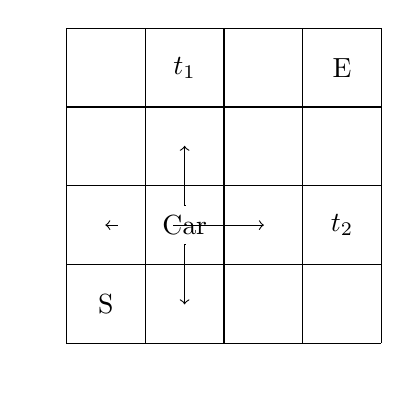
\begin{tikzpicture}[every node/.style={minimum size=1cm-\pgflinewidth, outer sep=0pt}, arrow/.style={thick}]
    \draw[step=1cm,color=black] (-2,-2) grid (2,2); 
    \node[](start) at (-1.5, -1.5) {S};
    \node[](end) at (1.5, 1.5) {E};
    \node[](car) at (-0.5, -0.5) {Car};
    
    \node[](car_up_center) at (0.0, -0.25) {};    
    \node[](car_up) at (-0.5, 1.0) {};
    
    \node[](car_down_center) at (0.0, -0.75) {};
    \node[](car_down) at (-0.5, -2.0){};

    \node[](car_left_center) at (-1.35, -0.5) {};
    \node[](car_left) at (-2.0, -0.5){};

    \node[](car_right_center) at (-0.65, -0.5) {};
    \node[](car_right) at (1.0, -0.5){};
    
    \node[](charge site) at (-0.5, 1.5) {$t_{1}$};
    \node[](charge site) at (1.5, -0.5) {$t_{2}$};
    \draw[->, to path={-| (\tikztotarget)}]
 	( car_up_center) edge (car_up)  (car_down_center) edge (car_down) ;
     \draw[<-, to path={-| (\tikztotarget)}]
 	(car_left) edge (car_left_center) (car_right) edge (car_right_center);
\end{tikzpicture}
\caption{场景3:电动车路径规划问题的网格地图,其中 $t_1, t_2$分别表示两个充电桩的位置}
\end{center}
\end{figure}

\section{本章小结}
作为本文的正式内容的第一个章节,我们给出了路径规划问题的定义,以及出现的多个新的场景和需求。通过给出严格定义,将为下面章节我们使用强化学习解决问题提供较好的支持。

% \subsection{场景4:动态地图环境}
% 在现实交通网络环境中,另外一个影响路径规划算法的问题为道路堵车问题,而城市道路堵车状况可以被建模为一种依赖于时间规律变化的场景。正如在1.2节提到的路径规划问题的分类,我们可以将这一问题划分到动态图或具有时序依赖的路径规划范畴中。在这个场景中,我们将基于场景1的任意一条边的行驶损耗建模成一个依赖于时间周期性变化的函数,并且使用一天作为变化的一个周期来模拟城市的堵车状态。这使得我们的路径规划算法在考虑行驶路径最短的情况下,需要考虑在不同时段下,不同路段堵车情况所带来的额外损失以求得依赖于时序的最短路径。\par
% 首先对任意一条图上的边$e_{i,j}$,我们定义重新定义场景1的函数为一个基于正太分布函数$f_{e_{i,j}}(t) = a\times N(\mu, \sigma^2) + C$,
% 表示其依赖时序变化的损耗值,我们需要针对每条边设计其参数$a, b, \mu, \sigma$的值。接下来我们将简单的构建一个典型的城市堵车状况,即在上班时段,大多车辆从城市周围进入城市中心,在下班时段,大多数车辆从城市中心向城市四周分布行驶。\par
% 因此我们首先定义城市中心位置为 $v_center$,对$v_i\in V, v_i \neq v_center$,根据二维几何空间欧氏距离的定义,其到中心的距离表示为 $D(v_center, v_i)$。我们对任意一条边$e_{i,j}$通过计算其是否使得车辆在通过它后是否远离中心分为两类$\{toWork, offWork\}$。当车在通过边$e_{i,j}$,即从点$v_i$到达$v_j$后,我们通过如下公式:
% \begin{center}
% \begin{equation}
% e_{i,j} is \begin{cases}
% toWork &\mbox{if $D(v_{center}, v_i)\leq D(v_{center}, v_j)$}\\
% offWork &\mbox{if $D(v_{center}, v_i) > D(v_{center}, v_j)$}
% \end{cases}
% \end{equation}
% \end{center}
% 现在我们按照24小时为周期,定义7-9时刻为上班高峰期,17-19为下班高峰期。通过预先定义的$v_center, \mu_{toWork}, \sigma_{toWork}, \mu_{afterWork}, \sigma_{afterWork}, a, b$,,以及用$MaxDistance$表示到中心点最远点的距离。推算出其他边的参数值。然后我们按照如下算法流程设计图计算某条边的的损耗函数的参数值。


% \begin{algorithm}[H]
%     % \DontPrintSemicolon
% 	\KwIn{G=$\{V, E\}$,\quad$v_{center}$,\quad$\mu_{toWork}$, \quad $\sigma_{toWork}$, \quad $\mu_{afterWork}$, \quad  $\sigma_{afterWork}$, \quad  $a$, \quad  $b$, \quad $MaxDistance$}
% 	\KwOut{$\sigma_{1..n}, \mu_{1..n}, a_{1..n}, b_{1..n}$}
% 	Inlization\;
% 	\Begin{
%         $\mu_{toWork} \leftarrow 8$,\;
% 	    $\sigma_{toWork} \leftarrow 1$,\;
%         $\mu_{afterWork} \leftarrow 18$,\;
%  	    $\sigma_{afterWork} \leftarrow 1$,\;
%  	    $a \leftarrow A, A > 0$,\;
%         $b \leftarrow B, B > 0$\;
% 	}
% 	\For{each edge $e_{i,j} \in E$}{
% 	    \If{$D(v_{center}, v_i)\leq D(v_{center}, v_j)$}{
% 	    $\mu_{e_{i,j}} \leftarrow \mu_{toWork} \times \frac{D(v_{center}, v_i)}{MaxDistance}$,\;
% 	    $\sigma_{e_{i,j}} \leftarrow \sigma_{toWork} \times \frac{D(v_{center}, v_i)}{MaxDistance}$,\;
% 	    }
% 	    \Else{
% 	    $\mu_{e_{i,j}} \leftarrow \mu_{offWork} \times (1 + \frac{D(v_{center}, v_i)}{MaxDistance})$,\;
% 	    $\sigma_{e_{i,j}} \leftarrow \sigma_{offWork} \times \frac{D(v_{center}, v_i)}{MaxDistance}$,\;
% 	    }
% 	}
% \caption{城市道路堵车模拟算法}
% \end{algorithm}

\end{document}
\documentclass{standalone}
% preamble: usepackage, etc.
\begin{document}

\chapter{基于搜索的路径规划方法}
\section{Dijkstra 算法}
\section{$A^{*}$ 算法}
\section{相关改进算法}
\end{document}
\documentclass{standalone}
% preamble: usepackage, etc.
\begin{document}

\chapter{强化学习基础}

强化学习是一种学习如何进行控制和决策的框架,强化学习的灵感来自于仿生学,它完成了从当前的环境状况到行为的映射,并通过学习这一映射过程使得从环境中得到的奖赏值最大化。这样一种框架被誉为可能是发展为强人工智能的框架,包括博弈论、控制理论、群体智能、多智能体系统等领域都与强化学习可以进行结合和交叉。在控制领域,强化学习被视为一种拟合动态规划方法。在博弈论领域,它被用来解释均衡点的出现及其原因。它和有监督学习,无监督学习组成了机器学习领域三个基本的学习框架。它不同于有监督学习和无监督学习,原因在于,在强化学习中,并不存在类似于有监督学习中的标签信息,只有奖赏信号用于指导整个学习过程,同样这也不同于无监督学习中没有任何信号和标签指导学习过程。\par

\section{智能体建模方法和马尔科夫决策过程}
强化学习框架的设计一般基于智能体建模的方式实现,基于智能体的模型是一种为了模拟控制和交互的计算模型,这样一种框架包括智能体和环境两类主体,其在多个领域都有广泛的应用,如在生物学中用于研究种群的分布,人口变化等问题,在经济和社会学中,用于研究城市人口流动和城市规划问题,消费者行为分析等。在强化学习中,我们通过图4-1所示的框架对强化学习进行建模。
\begin{figure}[h]
	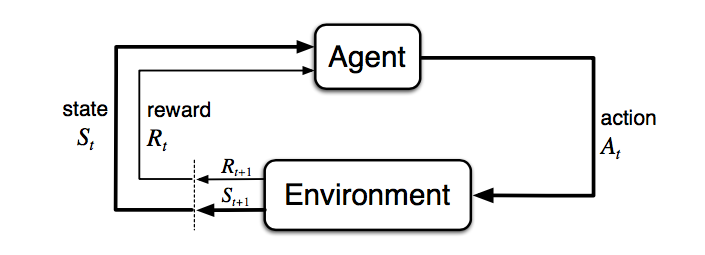
\includegraphics[width=12.0cm]{pic/4-1.png}
	\caption{强化学习框架}
	\label{4-1}
\end{figure}
\section{强化学习}

\subsection{价值函数}
\subsection{策略函数}
\subsection{基于价值函数的方法}
\subsubsection{查表法}
\subsubsection{函数近似法}

\subsection{基于策略梯度的方法}

\end{document}
\documentclass{standalone}
% preamble: usepackage, etc.
\begin{document}
	
\chapter{基于强化学习的路径规划算法}
在这一章我们将给出用于路径规划问题的强化学习算法的描述,包括了首先将了路径规划这一图论问题转化到马尔科夫决策过程使得我们可以应用强化学习。其次我们针对多个不同的场景设计了不同的算法,我们将介绍这些算法,同时给出这样设计的原因。\par
传统的路径规划算法对待该问题的形式为,在预处理阶段,首先在图上按照算法进行一定的计算和结果的存储,如存储两点间的最短路径距离,路径经过的节点等信息,也有部分较复杂的算法,对其做缩点等图上的优化操作等,第二步进入查询阶段,即根据用户给定的起点和重点,通过预处理得到的结果再给出最终的最短路径规划结果。这一建模方法并不是一个典型的强化学习建模方式,因此在应用到强化学习到该问题时,我们需要变换问题的形式为,在给定某个地图后,我们先经过一个强化学习算法学习过程,例如 Q-leanring 方法,得到一个最优的策略函数和价值函数,这一步等同于传统算法的预处理阶段,第二步,对于查询,我们直接将学习到的策略部署到用户端。在任意时刻,给定当前的状态,给出选择后的行为,因此规划过程变成了在线过程,而非离线。同样如果需要达到离线规划的效果,我们需要该策略对应环境下的模拟环境,通过给定初始状态和模拟环境,得到完整的规划路径后返回结果给用户。具体的流程如图 xxx 所示。在我们的方法中,我们只关注相关算法的设计,因此对于一个完整的路径规划系统的设计不在我们的研究范畴。\par
在算法上,我们设计了一个端到端的系统,即模型的决策系统输入为环境的原始状态,输出也为环境的原始行为。端到端的设计具有以下几种优势,首先其使得我们的模型更易于优化,如果我们将模型拆分成多个子模块,那么对于每个模块我们需要单独设计其优化算法,这大大增加了算法的设计和调试难度。其次通过端到端的模型,更能发挥机器学习的能力,在早期的人工智能领域,因为限于当时的计算能力和数据量,比较流行的算法往往加入了大量的人类的先验,但随着计算能力的快速提高,大数据的出现,端到端的模型因此展现出了巨大的能力,在多个领域和问题张获得了非常好的结果。因此在我们的算法中,我们也将采用端到端的设计。\par

\section{基于马尔科夫决策过程的算法形式表述}
在这一节,我们将路径规划问题表述为一个建立在离散时刻上的马尔科夫决策过程,给出其状态空间$S$,行为空间$A$,状态转移函数$P$,奖赏函数$R$等马尔科夫决策过程的几个基本元素的定义。然后针对不同的场景,我们提出了基于
Q-leanring 的算法。针对每个不同的场景,我们对算法做了相应的调整,并给出这样设计的思路和原因。\par
通过使用网格地图作为我们的环境,比较易于将智能体在任意一个状态下的行为选择规约到一个固定的状态集合上,如果不按照此建模方式,我们需要提出一个更灵活的对行为和状态建模的方式,而非端到端的方式,关于这一方向的讨论我们将在最后一章总结和未来方向中进行讨论。

\section{不同场景下算法设计方法}
在这一章,我们定义四个场景的对应马尔科夫决策过程的严格定义,同时给出相应的算法。第二,三,四个场景都部分的基于场景一,然后同时根据场景的特性,做了相应的更改。我们希望四个场景能尽可能多个共享相同的建模上的设计,这样使得算法设计能够具有更好的通用性使得其并不被完全限制于该场景下,以及更进一步的,提出一个单一的集合模型使得其能够同时解决多个场景下的规划问题。
\subsection{场景一:简单网格地图}
首先对于一个简单的$N \times M$大小的网格地图,由于在任意时刻,车辆可以在不超出地图边界的情况下向上下左右四个方向移动,同时不考虑任何对车辆的行驶限制。因此对该场景的状态定义为$s_t = (x_t^car, y_t^car, x^{target}_t, y^{target}_t), x_t^car=0..N-1, y_t^car=0..M-1, x^{target}_t=0..N-1, y^{target}_t=0..M-1$, 其中$x_t^car, y_t^car$表示车辆当前位置,$x^{target}_t, y^{target}_t$ 表示目标位置。其行为定义集合为$a_t \in {Up, Down, Left, Right}$分别表示向上,下,左,右行驶。对于状态转移$P{s_{t+1}|s_t, a_t}$设计,我们限制车辆每个时刻只能移动一个单位的距离,同时不能超出边界,因此将状态转移表述为一个确定性过程,同时我们需要特殊判断是否车辆会超出地图边界,如果超出,维持原状态。定义公式如下:
\begin{center}
    \begin{equation}
    s_{t+1} = \begin{cases}
    (x_t^car, y_t^car, x^{target}_t, y^{target}_t) &\mbox{if car will reach out of map}\\
    (x_t^car + 1, y_t^car, x^{target}_t, y^{target}_t) &\mbox{if $a_t$ is Right}\\
    (x_t^car - 1, y_t^car, x^{target}_t, y^{target}_t) &\mbox{if $a_t$ is Left}\\
    (x_t^car, y_t^car + 1, x^{target}_t, y^{target}_t) &\mbox{if $a_t$ is Up}\\
    (x_t^car, y_t^car - 1, x^{target}_t, y^{target}_t) &\mbox{if $a_t$ is Down}
    \end{cases}
\end{equation}
\end{center}
奖赏函数的设计是强化学习中一个核心的部分,特别是对于给定的场景本身不存在一个原有的奖赏产生机制时,我们需要手动设置和调整奖赏函数的设计,作为唯一指导智能体进行学习的信号,我们需要将我们的学习目标或评价机制通过奖赏函数体现出来。而设计奖赏函数需要遵循以下几个原则,首先奖励函数不能是过于稀疏的,过于稀疏的奖赏函数,即在大多数状态空间的点上为0,会使得智能体在初始探索时,难以获得有效的指导信号。因为智能体需要根据不同状态下奖赏值的大小进行行为的选择和策略的更新,而稀疏的奖赏函数导致了在初期探索过程中无法进行更新,特别在一些函数近似的方法中,如使用深度神经网络拟合方法时,参数的更新无法获得有效的梯度方向信息,导致模型参数无法收敛,甚至振荡和爆炸。其次,奖赏函数的设计不应该体现任何关于策略的指导信息,即我们不应该直接将智能体期望学习到的策略融入到奖赏信号中,例如如果为围棋问题设计奖赏信号,最直观和符合原则的做法为只有当达到获胜状态时才给予一个正的奖赏信号,而在其他状态下不产生任何奖赏信号。因此基于这两个原则,我们设计奖赏函数基于三个部分,首先如果在一步的移动中,智能体更加接近目标点,我们给+1的奖励,如果远离则为-1的奖励,如果动作导致其行驶出地图边界,我们给-10的奖励,如果新的状态到达了目标点,我们给予+100的奖励。因此对场景1的奖赏函数公式$R_{case1}$定义如下:
\begin{center}
    \begin{equation}
    r_t(s_t, s_{t+1}, a_t) = \begin{cases}
     sng(Distance(x_{t+1}^car, y_{t+1}^car, x^{target}_{t+1}, y^{target}_{t+1}) - Distance(x_t^car, y_t^car, x^{target}_t, y^{target}_t)) + 100 and return terminal signal&\mbox{if car get the target point}\\
     sng(Distance(x_{t+1}^car, y_{t+1}^car, x^{target}_{t+1}, y^{target}_{t+1}) - Distance(x_t^car, y_t^car, x^{target}_t, y^{target}_t)) - 10 &\mbox{if car try to reach out of map}\\
     sng(Distance(x_{t+1}^car, y_{t+1}^car, x^{target}_{t+1}, y^{target}_{t+1}) - Distance(x_t^car, y_t^car, x^{target}_t, y^{target}_t))&\mbox{else}\\
     \end{cases}
    \end{equation}
\end{center}
完成了对场景的马尔科夫决策过程的定义,我们采用基于查表法的 Q-learning 的强化学习算法解决这一问题,原因在于该场景的状态和行为的维度较低,因此适合使用查表法,状态行为价值函数,即 Q 函数的规模为$4\cdotN^2M^4$。对于 Q-learning 中学习速率的设置,由于该场景为一个静态场景,因此我们将速率设置在较大的范围进行调参,以保证模型以较少的数据量即可收敛。
\subsection{场景2:带有转弯惩罚的场景}
场景2中,我们加入了额外的转弯惩罚,使得例如似在场景1中,如果智能体探索出了多个最短路径,但选择较少左转或掉头,更多选择直行和右转的最短路应该是更优的。对该场景下的马尔科夫决策过程建模,状态$s_t$和$a_t$,以及状态转移矩阵$P(s_{t+1}|s_t, a_t)$我们都与场景1保持相同。但我们的奖励函数需要体现我们的场景变化,即对如果智能体选择了左转或掉头的动作,我们需要加入额外的惩罚。因此对场景2的奖赏函数$R_{case2}$定义如下:
\begin{center}
    \begin{equation}
    r_t(s_t, s_{t+1}, a_t) = \begin{cases}
     R_{case1}(s_t, s_{t+1}, a_t) - 5 &\mbox{if the car choose turn left or turn around}\\
     R_{case1}(s_t, s_{t+1}, a_t) &\mbox{else}
     \end{cases}
    \end{equation}
\end{center}
同样由于$s_t, a_t$的形式和规模相比场景1未发生变化,我们仍然沿用基于查表法的 Q-learning,并设置一个较大的学习速率进行更新。
\subsection{场景3:带有行驶路径限制和充电桩的场景}
在第三个场景下,我们设计了基于电动车的路径规划算法。基于电动车的路径规划问题的特点为我们需要考虑汽车的行驶路径限制。电动车相比传统汽油车的单次行驶路径较短,因而导致对于这一特殊场景的出现,相应的我们需要对该场景下的马尔科夫决策过程进行一定的修改以适应该场景。\par
首先我们需要定义场景中有$k$个充电桩,其位置组成的序列为$chargeSite = (x_1^{site}, y_1^{site}, x_2^{site}, y_2^{site}, ... , x_k^{site}, y_k^{site})$,同时定义智能体的当前剩余能量为$power_t$,以及车辆的满电量值为$FULL\_POWER$,在每次车辆到达充电桩后,其当前电量都会被赋值为满电量值。基于以上定义,对该场景下的状态定义为:
\begin{center}
    \begin{equation}
        s_t = (x_t^car, y_t^car, x^{target}_t, y^{target}_t) \union chargeSite \union
    \end{equation}
\end{center}
对行为$a_t$的定义维持不变。对状态转移函数,我们需要考虑在车辆在电量耗尽且未到达充电站或目标点时返回一个结束信号。因此状态转移公式$P_{case3}$如下:
\begin{center}
    \begin{equation}
    s_{t+1} = \begin{cases}
    (x_t^car, y_t^car, x^{target}_t, y^{target}_t, power_t-1, chargeSite) &\mbox{if car will reach out of map}\\
    (x_t^car + 1, y_t^car, x^{target}_t, y^{target}_t, power_t-1, chargeSite) &\mbox{if $a_t$ is Right}\\
    (x_t^car - 1, y_t^car, x^{target}_t, y^{target}_t, power_t-1, chargeSite) &\mbox{if $a_t$ is Left}\\
    (x_t^car, y_t^car + 1, x^{target}_t, y^{target}_t, power_t-1, chargeSite) &\mbox{if $a_t$ is Up}\\
    (x_t^car, y_t^car - 1, x^{target}_t, y^{target}_t, power_t-1, chargeSite) &\mbox{if $a_t$ is Down}
    \end{cases}
    \end{equation}
    \mbox{其中对$power_{t+1}$的转移公式$P(power_{t+1}| powert_{t}, x_{t+1}^{car}, y_{t+1}^{car})$定义如下:}
    \begin{equation}
        power_{t+1} = \begin{cases}
        return terminal signal &\mbox{if $power_t \leq 0$}\\
        FULL\_POWER &\mbox{if (x_{t+1}^{car}, y_{t+1}^{car}) is a charge site}\\
        power_{t} - 1 &\m{else}
        \end{cases}
    \end{equation}
\end{center}
对奖赏函数的设计,我们加入中途耗尽电量的惩罚和到达充电桩的奖赏值。因此对奖赏函数$R_{case3}$更新如下:
\begin{center}
    \begin{equation}
    r_t(s_t, s_{t+1}, a_t) = \begin{cases}
     R_{case1}(s_t, s_{t+1}, a_t) - 100 &\mbox{if the car out ot power in the middle}\\
     R_{case1}(s_t, s_{t+1}, a_t) + 20&\mbox{if car reach the charge site}\\
     R_{case1}(s_t, s_{t+1}, a_t)&\mbox{else}
     \end{cases}
    \end{equation}
\end{center}
在该场景中,我们的算法仍然沿用基于查表法的 Q-leanring 算法,状态行为价值函数的空间规模为$4\cdot MAX\_POWER\cdot N^{2+k}M^{2+k}$。但如果在$k$较大的情况下,即充电桩数目过多时,可以考虑使用基于函数近似的方法。
\subsection{场景4:动态地图环境}
在场景4中,我们将地图的损耗变为随时间动态变化的函数,
to be done1!!!
\subsection{本章小结}
\end{document}
\documentclass{standalone}
% preamble: usepackage, etc.
\begin{document}
	
\chapter{代码实现及实验}
在本章,我们将给出基于强化学习的路径规划问题的算法实现,以及实验结果展示。首先我们介绍为实现该算法,我们设计并开发了一个基于 Python 的强化学习框架,其包括了 Q-leanring 等多个方法,同时我们实现了多个场景下的地图环境,然后给出我们的实验设计和参数的设置。其次我们给出实验的结果,以及对结果的简要分析。
\section{基于面向对象设计的代码实现}
在代码实现上,我们基于 Python语言实现了基于面向对象设计思想的代码框架,以期望代码能够具有较高的鲁棒性和重用性和灵活性。\par
首先在类的设计上,我们将智能体抽象为代码中的 Agent 类,环境抽象为Environment 类,两者都是一个抽象类(Abstract Class),其次,我们将任何一种算法抽象为 Model 类(同样为抽象类),通过分离智能体和模型类,可以使得智能体方便载入各种不同的算法,并保持自身行为方式不改变,这使用了设计模式中的典型的策略模式(Strategy Pattern)。同时我们设计了Config 类用于托管各个模块的配置文件,超参数等,这些参数在实验开始时通过本地的文件加载进来,这使得我们解除了所有的硬编码(Hard Code),使得对实验的调参工作只需要更改配置文件即可实现,从而变得相对容易和灵活。同时,我们设计了一个 Sampler 的类。它将托管智能体与环境的交互过程,即采样过程,这使得我们能通过实现不同的 Sampler 类,轻松的更改对采样过程的控制。整个代码的UML图如下:
\begin{figure}[H]

	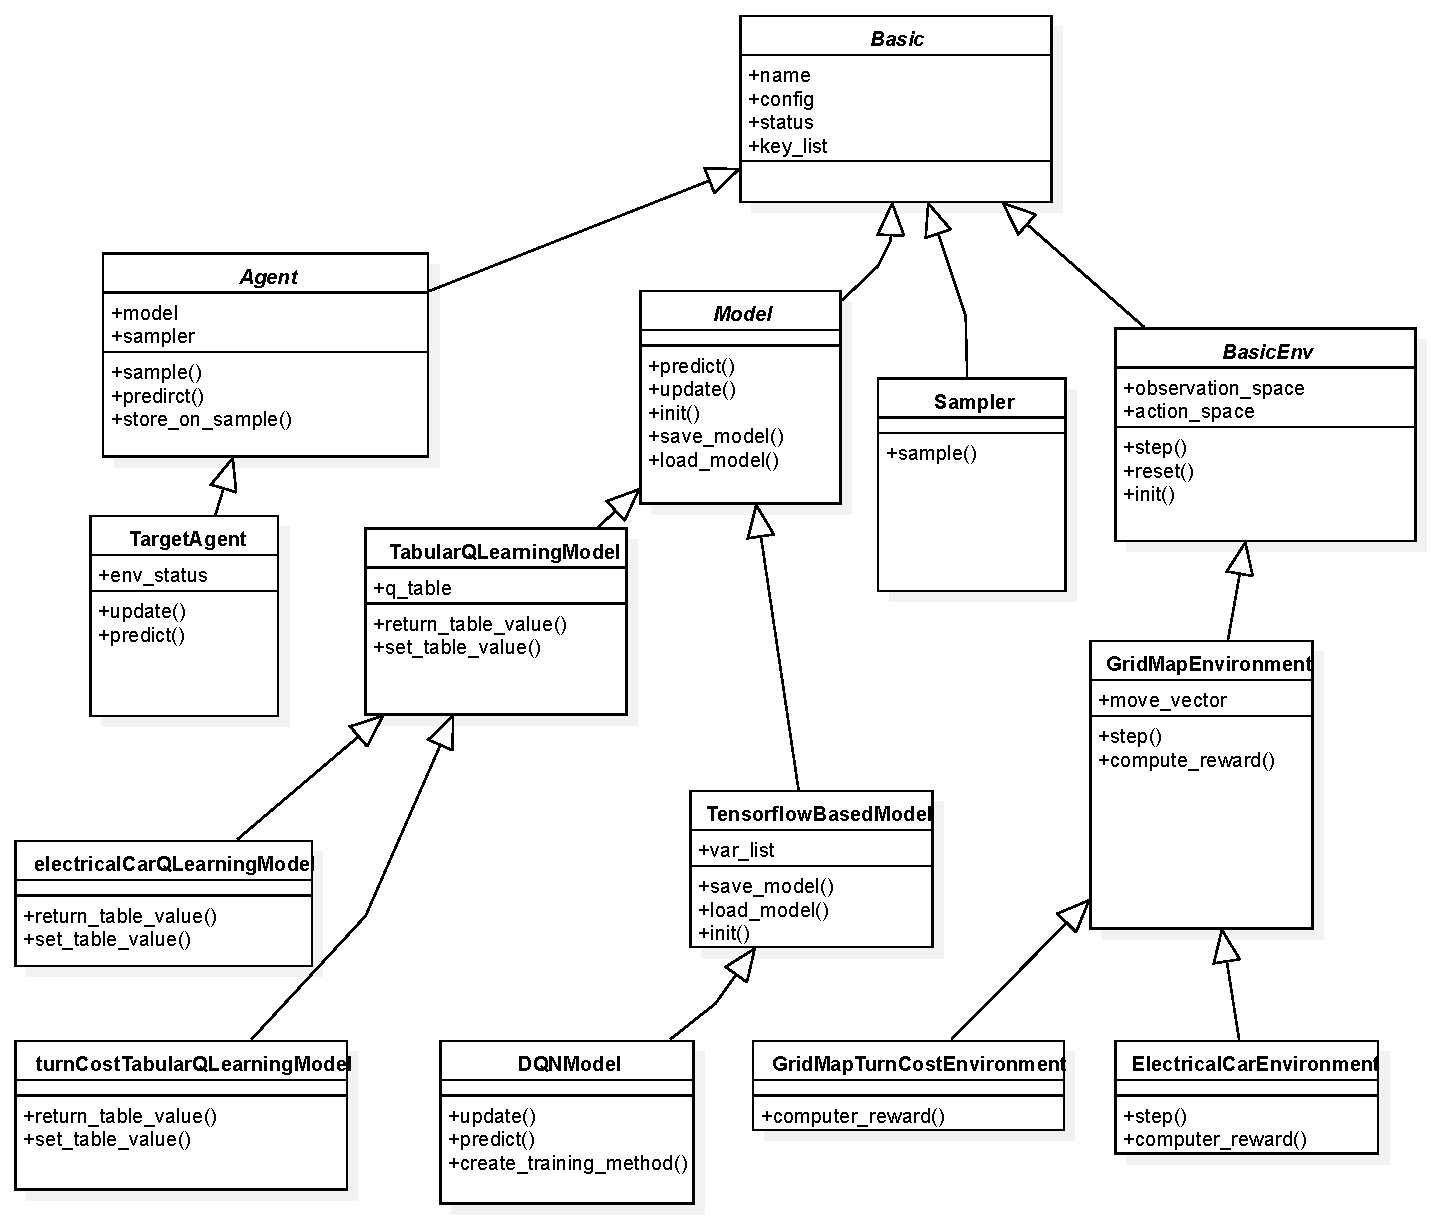
\includegraphics[width=12.0cm]{pic/6-1.pdf}
	\caption{代码实现 UML 图}
	\label{6-1}
\end{figure}

对于实验过程的监视和结果的存储,我们同样进行了一个自上而下的设计方法,所有代码中的类都继承自一个基类Basic,这使得我们方便管理所有模块在训练过程中数据和结果的保存等。自上而下的方法是指所有的结果和数据的存储动作,都是从最高层的模块开始,每个模块管理自身内部的子模块。即从智能体和环境连个作为最高层的模块分别触发这一动作后,智能体会调用自身模型,即算法部分的数据和结果保存动作,然后依次向下。同样我们在 Basic 中设计了status\_key 这一属性,使得模型可以根据不同的状态将数据和结果存储在不同的文件下,典型的例子为智能体在训练和测试过程中的奖赏函数值通过设置该属性值被分别存储在两个文件。
\section{实验设置和结果}
在这个小节中,我们给出了实验的详细设置以及细节,包括了环境相关设置,超参数设置,然后给出可视化的结果和图标等。在三个实验中,为了避免随机性带来的不稳定性和结果的不准确性,我们在相同的参数设置下,设置不同的随机种子后运行了10次独立实验,并将10次独立实验的平均值作为我们最后的结果展示。通过多次独立实验可以保证实验结果的稳定性和更可靠性。
\subsection{场景1}
在该实验下,我们设置地图大小为$4x4$,即 $N=4, M=4$起点为$(0, 0)$,终点为$(3, 3)$。对智能体,加入了一个基于采样数据量指数衰减的$\epsilon-Greedy$探索策略,探索策略只在采样中使用,即行为策略中使用。$\epsilon$初始值为0.3,经过衰减后最终值为0.0,对于 Q-leanring 模型,由于场景固定目标点位置不变,所以实际使用的Q-learning 查找表的大小为$4\cdot N \cdot M$,学习速率设置为0.8。训练过程设置为,每次智能体采样100个点后,进行训练和更新模型一次,然后进行测试,测试时采样100个数据点,统计出现的100个点中完整的一个过程的累计奖赏值。整个过程迭代20次\par
智能体在测试时的收到的累计奖励函数图变化如图\ref{case1reward}所示:
\begin{figure}[H]
    \centering
    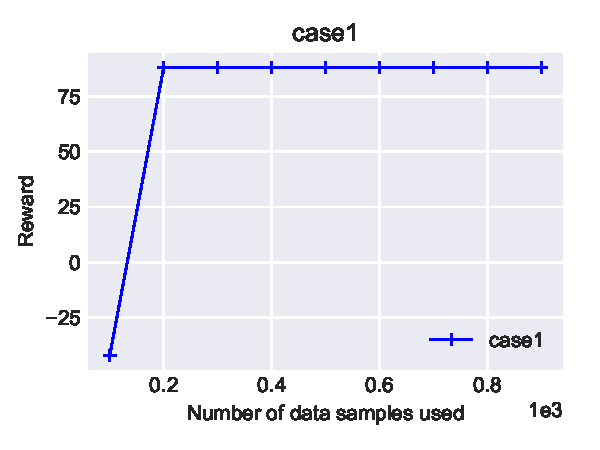
\includegraphics{pic/case1/case1.pdf}
    \caption{累计奖赏值曲线,虚化部分为曲线方差的上下界\\}
    \label{case1reward}
\end{figure}
可以看出,在两次采样和训练周期后,模型的奖赏值就收敛到了一个稳定的全局最优值,并且10次独立实验结果的统计方差几乎为0,说明结果的稳定性较高,结果可以稳定复现。同时我们将Q-leanring的查找表也做了可视化分析,进一步确认智能体学到一个实际有效的策略。首先我们选择了三个点$(0, 3), (2, 2), (0, 0), (3,0)$的对应4个行为的状态行为函数的变化过程,并进行分别进行比较。在起始点$(0,0)$时,显然向右或向上走优于其他行为,因为该情况下只有向左或向上为合法动作,所以向右和向上行的Q 值曲线较高,并且基本重合,如图\ref{1case00}所示。
在$(2, 2)$点时,四个动作都为合法动作,但明显向右或向上走更接近目标,因此此时采取向右或向上也应该具有更高的Q值,如图\ref{1case22}。在点$(3, 0)$和点$(0, 3)$,前者的最优动作为向上,后者为向右,对应的Q 值曲线也表明智能体学到了这一策略,如图\ref{1case30},和图\ref{1case03}所示。\par

\begin{figure}[H]
    \centering

	\subfigure[]{
		\label{1case00}
		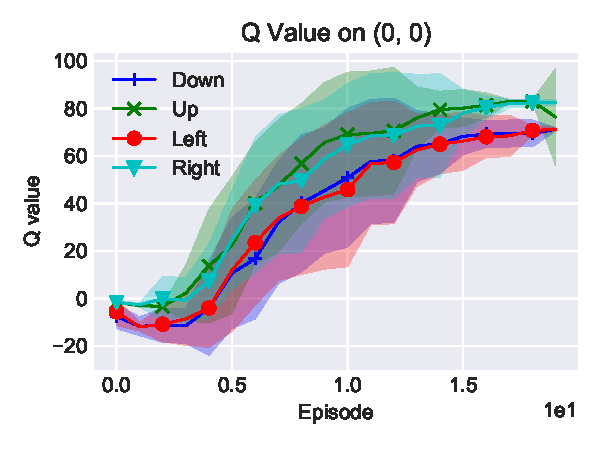
\includegraphics[width=7.3cm]{pic/case1/00.pdf}}
	\subfigure[]{
		\label{1case22}
		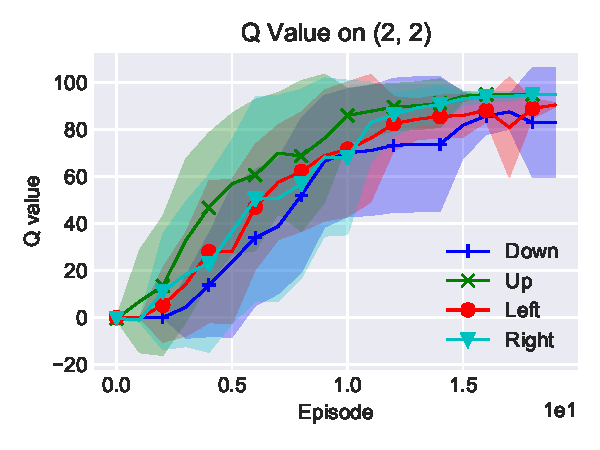
\includegraphics[width=7.3cm]{pic/case1/22.pdf}}
	\caption{Q 值在点(0,0)和点(2,2)的变化曲线}
	\label{fig1}
\end{figure}

\begin{figure}[H]
    \centering

	\subfigure[]{
		\label{1case30}
		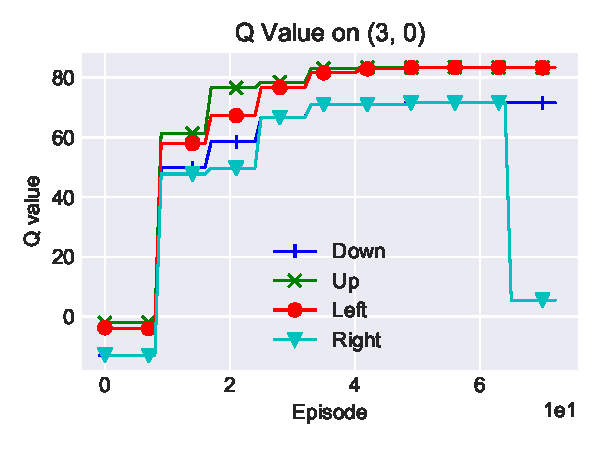
\includegraphics[width=7.3cm]{pic/case1/30.pdf}}
	\subfigure[]{
		\label{1case03}
		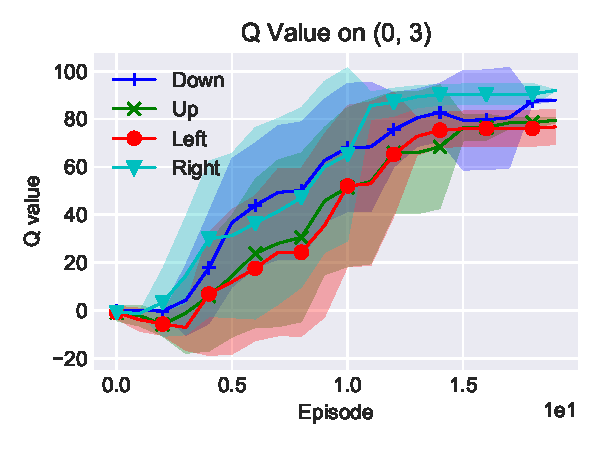
\includegraphics[width=7.3cm]{pic/case1/03.pdf}}
	\caption{Q 值在点(3,0)和点(0,3)的变化曲线}
	\label{fig2}
\end{figure}

\subsection{场景2}
在场景2中,我们的地图环境和场景1相同,但加入了额外的转弯损失,当智能体选择左转或掉头时,会得到额外的20的乘法。对于智能体,采用相同的$\epsilon-Greedy$策略和相同的参数设置。因为我们需要加入转弯的信息用于智能体决策,所以对应的 Q-leanring 的查找表的大小按照 xx 节的定义为$4^2 \cdot N\cdot M$,即加入额外的一维记录上一时刻的车辆方向的状态,使得智能体能够获得关于是否触发左转动作的信息。由于 Q-learning 的查找表规模变大,因此在实验中,我们将迭代次数增加为100次。如图\ref{case2reward}所示,展示了智能体在测试时的累计奖赏,可以看到模型稳定的收敛在了最优策略上。
\begin{figure}[H]
    \centering
    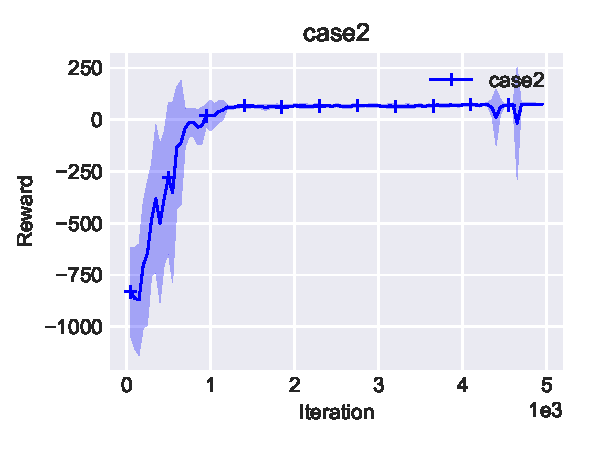
\includegraphics{pic/case2/case1.pdf}
    \caption{累计奖赏值曲线}
    \label{case2reward}
\end{figure}
简单分析可得,该场景下仅存在一个最优路径,如图\ref{case2res}所示:
\begin{figure}[H]
\begin{center}
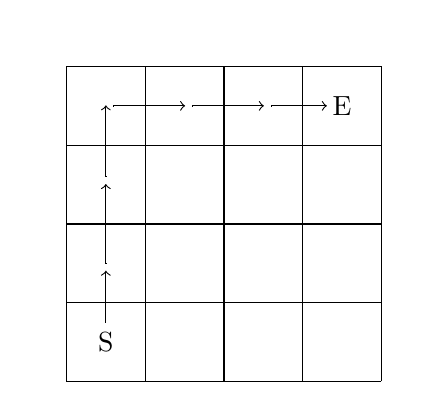
\begin{tikzpicture}[every node/.style={minimum size=1cm-\pgflinewidth, outer sep=0pt}, arrow/.style={thick}]
    \draw[step=1cm,color=black] (-2,-2) grid (2,2); 
    \node[](start) at (-1.5, -1.5) {S};
    \node[](end) at (1.5, 1.5) {E};
    \node[](start_up) at (-2.0, -1.25){};
    \node[](n11) at (-1.5, -0.1){}; 
  
    \node[](n1) at (-1.0, -0.5){}; 
    \node[](n2) at (-1.5, 1.0){};  
    
    \node[](n22) at (-1.0 ,0.6){}; 
    \node[](n3) at (-1.5, 2.0){};  
   
    \node[](n33) at (-1.4, 1.0){};  
    \node[](n4) at (0.0, 1.5){};  
    
    \node[](n44) at (-0.4, 1.0){};  
    \node[](n5) at (1.0, 1.5){};  
     
    \node[](n55) at (0.6, 1.0){};  
    \node[](n6) at (1.8, 1.5){};  

    \draw[->, to path={-| (\tikztotarget)}]
 	(start_up) edge (n11)  (n1) edge (n2) (n22) edge (n3);
     \draw[<-, to path={-| (\tikztotarget)}]
 	(n4) edge (n33) (n5) edge (n44) (n6) edge (n55);
\end{tikzpicture}
\caption{场景2的最优路径}
\label{case2res}
\end{center}
\end{figure}

类似场景1,现在我们对部分状态的状态动作价值函数可视化,我们展示在同一位置坐标下,不同的动作的 Q 函数在上一个时刻的4个动作上的均值,显然,在该场景下,右转和直行应当比左转具有更高的 Q 值。简单分析可知,该场景下仅存在唯一的最优策略为从起点(0,0)出发,向上到达(0,3)后,右转到达终点(3,3),这样避免了左转带来的额外消耗。所以在(0,0)点时,不同于场景1的向上行驶和向右行驶动作t具有较为接近的 Q 值,在该场景下向上显著高于向右,如图\ref{2case00}所示。然后我们检查当智能体处在(3,0)且上一时刻方向为向右时的Q值大小(此时状态的下标为(3, 0, 3)),即当智能体处在只能选择左转才能以最短路径到达时,检测是否会因为额外转弯的惩罚丢失掉最优策略,如图\ref{2case303}所示。类似的给出当状态为(2,3,0)时的 Q 值曲线,如图\ref{2case230}所示。根据曲线可以看出,在(3,0,3)状态下,即在上一个行为为向右时,智能体选择了向上的动作(对应产生了左转)。类似的,在(2,3,0)时,即上一个行为为向下时,智能体选择了向右的动作(对应产生了左转)。这表明智能体合理的学习到了在优先保证最短路径的情况下,再尝试减小左转带来的额外惩罚。
\begin{figure}[H]
    \centering

	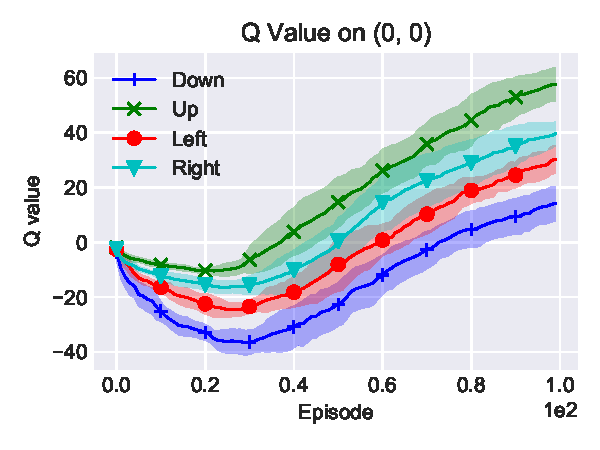
\includegraphics[width=7.3cm]{pic/case2/00.pdf}
    \caption{Q 值在点(0,0)时,并对上一时刻的行为求均值后的 Q 值曲线}
    \label{2case00}
\end{figure}


\begin{figure}[H]

	\subfigure[]{
		\label{2case303}
		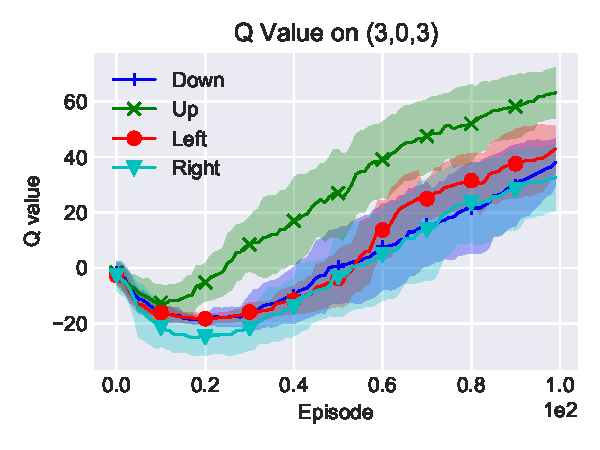
\includegraphics[width=7.3cm]{pic/case2/303.pdf}}
	\subfigure[]{
		\label{2case230}
		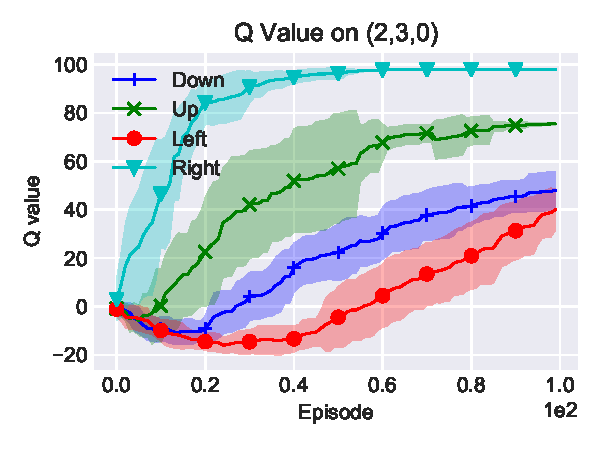
\includegraphics[width=7.3cm]{pic/case2/230.pdf}}
	\caption{Q 值在状态(3,0,3)和点(2,3,0)的变化曲线}
	\label{fig2}
\end{figure}

\subsection{场景3}
在该场景中,我们对环境分别在(1,2)和(3,1)加入了充电桩,其他的设置与场景1保持相同,同时对奖赏函数的设计做了如下设置,如果在中途电量耗尽则返回额外的40的惩罚,如果到达充电桩,返回2的奖赏值。设置车辆在满电量时的行驶距离为3,单次移动消耗1单位电量。对于智能体,我们需要加入两个充电桩的位置以及当前的剩余电量到状态中,因此 Q 函数查找表的规模为$4\times 3 \cdot N^3 \cdot M^3$。由场景的设置可知,该情景下最优路径如图\ref{case3best}所示。
\begin{figure}
    \centering
    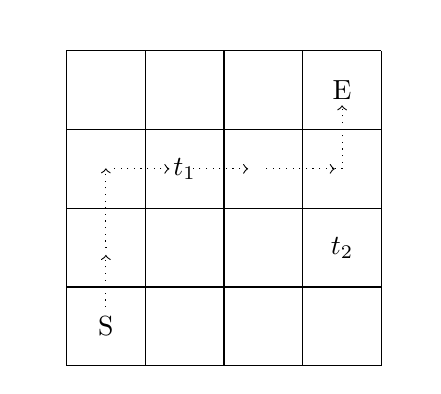
\begin{tikzpicture}[every node/.style={minimum size=1cm-\pgflinewidth, outer sep=0pt}, arrow/.style={thick}]
    \draw[step=1cm,color=black] (-2,-2) grid (2,2); 
    \node[](start) at (-1.5, -1.5) {S};
    \node[](end) at (1.5, 1.5) {E};
       
   \node[](charge site) at (-0.5, 0.5) {$t_{1}$};
   \node[](charge site) at (1.5, -0.5) {$t_{2}$};
   
    \node[](start_up) at (-2.0, -1.25){};
    \node[](n11) at (-1.5, -0.1){}; 
  
    \node[](n1) at (-1.0, -0.5){}; 
    \node[](n2) at (-1.5, 1.0){};  
    
    \node[](n22) at (-1.4 ,0.0){}; 
    \node[](n3) at (-0.2, 0.5){};  
   
    \node[](n33) at (-1.4, 1.0){};  
    \node[](n4) at (0.0, 1.5){};  
    
    \node[](n44) at (-0.4, 1.0){};  
    \node[](n5) at (1.0, 1.5){};  
     
    \node[](n55) at (0.6, 1.0){};  
    \node[](n6) at (1.8, 1.5){};  

    \draw[dotted, ->, to path={-| (\tikztotarget)}]
 	(start_up) edge (n11)  (n1) edge (n2);
     \draw[dotted, <-, to path={-| (\tikztotarget)}]
 	(n3) edge (n22);
	
	% path 1	
    \node[](p1_1) at (-0.4 ,0.0){}; 
    \node[](p1_2) at (0.8, 0.5){};  
    
    \node[](p1_3) at (0.5 ,0.0){}; 
    \node[](p1_4) at (1.9, 0.5){};  
    
    \node[](p1_5) at (1.9, 0.5){};  
       \node[](p1_6) at (1.5, 1.8){};  
      \draw[dotted, <-, to path={-| (\tikztotarget)}]
 	(p1_2) edge (p1_1)	(p1_4) edge (p1_3);

    \draw[dotted, ->, to path={-| (\tikztotarget)}]
 	     (p1_5) edge (p1_6);
    \end{tikzpicture}
    \caption{场景3的最优路径,虚线表示其为多个最优路径中的一个解}
    \label{case3best}
\end{figure}
首先我们给出智能体的测试环境下的累计奖赏值的曲线,如图\ref{case3reward}所示,可以看出智能体的策略收敛到了一个比较稳定的最优值。
\begin{figure}
    \centering
    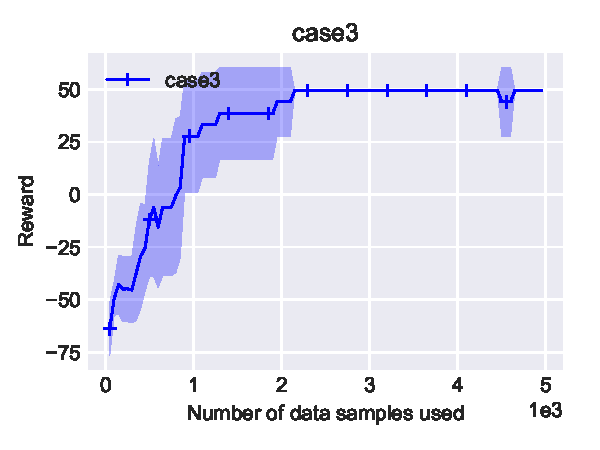
\includegraphics{pic/case3/case1.pdf}
    \caption{累计奖赏值变化曲线}
    \label{case3reward}
\end{figure}
同时我们检查智能体是否学习到了在自身电量不足以到达目标点时,能够寻找附近的充电桩,因此我们分别可视化了在点(0,2),(1,1),(2,2),(1,3),(2,1)以及(3,2)且电量值仅为1时的 Q 值变化曲线。在(0,2),(1,1),(2,2),(1,3)点,分别如图\ref{3case021},\ref{3case111},\ref{3case221},\ref{3case131},都通过选择对应的行为到达位于(1,2)的充电桩。对于点(3,2)如图\ref{3case321}所示,智能体选了了位于(3,1)的充电桩。同样我们检测了特殊的点(3,2),在该点下,在电量值为1的情况下,仍不需要进行充电即可直接达终点,如图\ref{3case321}所示。而智能体也很好的学习到了这一策略,未被奖赏函数中的到达充电桩带来的额外奖赏而干扰最短路径规划的结果。

\begin{figure}[H]
	\subfigure[]{
		\label{3case021}
		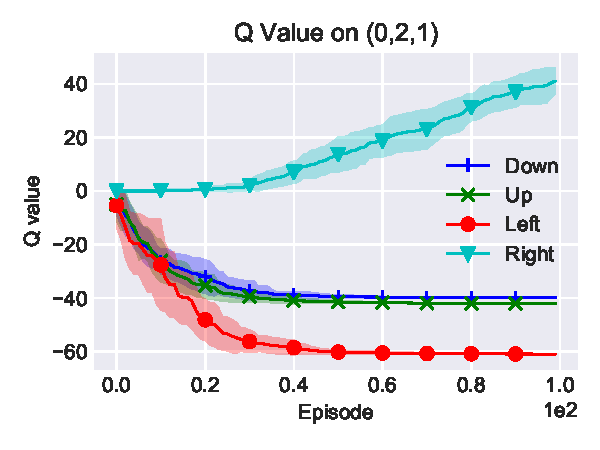
\includegraphics[width=7.3cm]{pic/case3/0,2,1.pdf}}
	\subfigure[]{
		\label{3case111}
		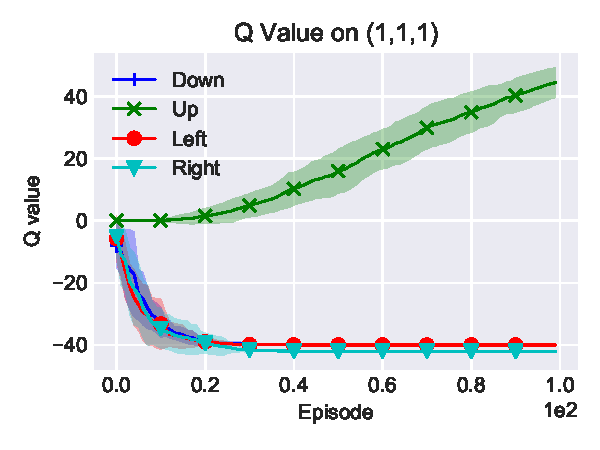
\includegraphics[width=7.3cm]{pic/case3/1,1,1.pdf}}
	   	\caption{Q 值在位置(0,2)和(1,1),且电量值为1时的变化曲线} 

	\label{fig2}
\end{figure}

\begin{figure}[H]
	\subfigure[]{
		\label{3case221}
		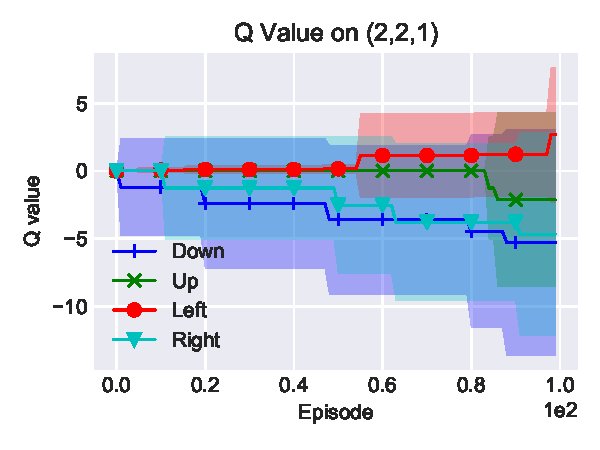
\includegraphics[width=7.3cm]{pic/case3/2,2,1.pdf}}
	\subfigure[]{
		\label{3case131}
		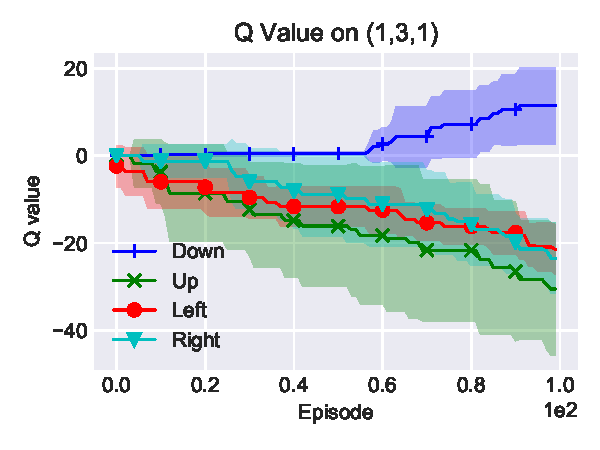
\includegraphics[width=7.3cm]{pic/case3/1,3,1.pdf}}
	\caption{Q 值在位置(2,2)和(1,3),且电量值为1时的变化曲线}
	\label{fig2}
\end{figure}

\begin{figure}[H]
	\subfigure[]{
		\label{3case211}
		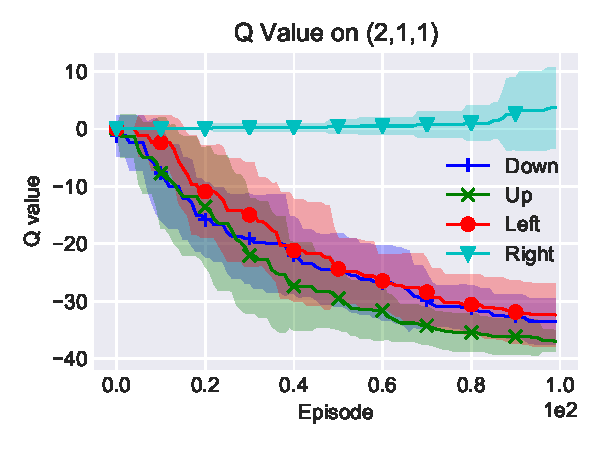
\includegraphics[width=7.3cm]{pic/case3/2,1,1.pdf}}
	\subfigure[]{
		\label{3case321}
		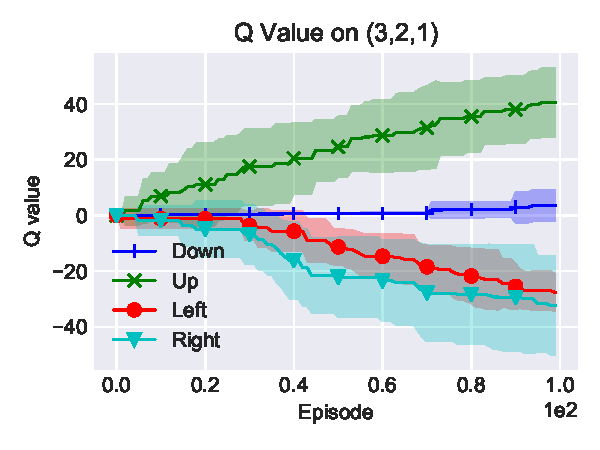
\includegraphics[width=7.3cm]{pic/case3/3,2,1.pdf}}
	\caption{Q 值在位置(2,1)和(3,2),且电量值为1时的变化曲线}
	\label{fig2}
\end{figure}
在训练过程中,在调整到达充电桩引起的额外奖赏值参数时我们发现,如果将该值设置过大,智能体容易陷入一个错误的最优策略,即通过反复的进出充电桩提高奖赏值,而我们通过调整这一值和到达终点的奖赏值的比例,使得智能体能够学习到正确的策略。
\section{本章小结}
在本章,我们给出了代码的实现细节,实验的参数设置和实验结果。通过实验结果的展示,验证了我们的算法实际学习到了合理的策略,表现出了其效果和有效性。同样在调参过程中我们发现了相应的问题,使得以后的相关研究可以进行借鉴参考。
\end{document}
\documentclass{standalone}
% preamble: usepackage, etc.
\begin{document}

\chapter{全文总结与展望}
\section{全文总结}
在该文中,我们设计并实现了基于强化学习的路径规划算法。我们首先引入了路径规划问题的定义和相关扩展,然后介绍了基于搜索的传统方法,并简单分析了其局限性。随后我们介绍了强化学习的相关背景,例如马尔科夫决策过程,智能体建模方法,最后详细给出了强化学习的 Q-learning 算法。在五章,我们给出了我们的算法,包括如何将路径规划问题转化为一个标准的强化学习环境,然后对要解决的三个场景分别提出了基于 Q-learning 的算法,给出了相关的定义和算法流程。在第六章,我们给出了实验的实现细节,包括了代码设计的核心思路和用到的设计模式。然后给出实验参数设置和实验结果,通过实验结果可以看出我们的算法很好的解决了相应的场景。\par
通过模型设计和实验结果的展示,可以看出,基于强化学习的路径规划算法相对传统的基于图上的搜索方法具有较大的优势。其强大的灵活性可以适应多种的场景,我们只需要调整相应的马尔科夫决策过程的形式,特别是奖赏函数的设计,即可完成对不同场景的路径规划算法设计,而传统的方法对不同的场景难以提出一个统一算法模型。
\section{后续工作展望}
在我们的工作中,我们的算法解决了小规模地图下的多个场景下的路径规划问题,但在现实路径规划系统中,问题的规模远远大于我们的实验设计,因此如何将我们的算法迁移到大规模场景下是未来的研究方向之一,这首先将影响到我们算法的设计,基于查表法的 Q-leanring 难以处理如此大规模的数据,因此可以在接下来的研究中通过基于函数近似的方法,利用神经网络等方法,例如 DQN 等近些年提出的深度强化学习算法解决该问题。结合强大的计算能力和大规模的神经网络,这类方法能够处理更加复杂的路径规划问题\par
第二的方向为,如何设计一个基于强化学习的通用的路径规划算法,在我们的工作中,虽然解决了部分场景,算法并不属于同一个框架,在部分设计上存在不同的地方,虽然相比传统方法已经具有很高的灵活性,但也在一定程度上限制了强化学习方法的进一步应用,因此在未来的研究中,可以关注如何设计更加灵活的状态,行为和奖赏函数以使得模型的泛化能力提高。\par
第三,如何设计一个离线算法也是未来的研究方向之一。我们的模型现在只能给出在线的规划算法,但常见的路径规划系统往往具有离线规划的能力,即单次询问即可给出完整的规划结果,所以如果把强化学习实际应用到现实系统中,如何实现离线规划也是重要的研究方向。\par
最后,在基于环境交互进行学习的同时,如何利用现有的行驶数据进行学习以及如何解决仿真环境与真实环境的差别而对模型训练引入的误差也是未来的重要的研究方向,这也不仅仅是该问题上的发展方向,也是强化学习该领域的一个重要方向。如果能很好的利用现实世界采集的真实数据,会大大降低模拟环境的误差带来的问题,提升模型的效果。
\end{document}
%\documentclass{standalone}
% preamble: usepackage, etc.
\begin{document}
	
\chapter{template}
This is the template of the chapter in split file.

\end{document}

% misc
\documentclass{standalone}
% preamble: usepackage, etc.
\begin{document}

\thesisacknowledgement
首先感谢我的导师郭宏亮教授,对我的毕业论文做出的指导和帮助。感谢我的家人,同学和朋友对我的帮助和支持。也感谢自己在毕业设计上所付出的努力,希望能给大学四年画上圆满的句号。
\end{document}
\thesisloadbibliography[nocite]{reference}

%
% Uncomment following codes to load bibliography database with native
% \bibliography command.
%
% \nocite{*}
% \bibliographystyle{thesis-uestc}
% \bibliography{reference}
%

% comment while no need
\documentclass{standalone}
% preamble: usepackage, etc.
\begin{document}

\thesisappendix

\end{document}
\thesisloadachievement{publications}
\documentclass{standalone}
% preamble: usepackage, etc.
\begin{document}

\thesistranslationoriginal
\section{Comparison of the Q-Routing and Shortest Path Routing Algorithms}

\begin{figure}[H]
    \centering
    \makebox[0pt]{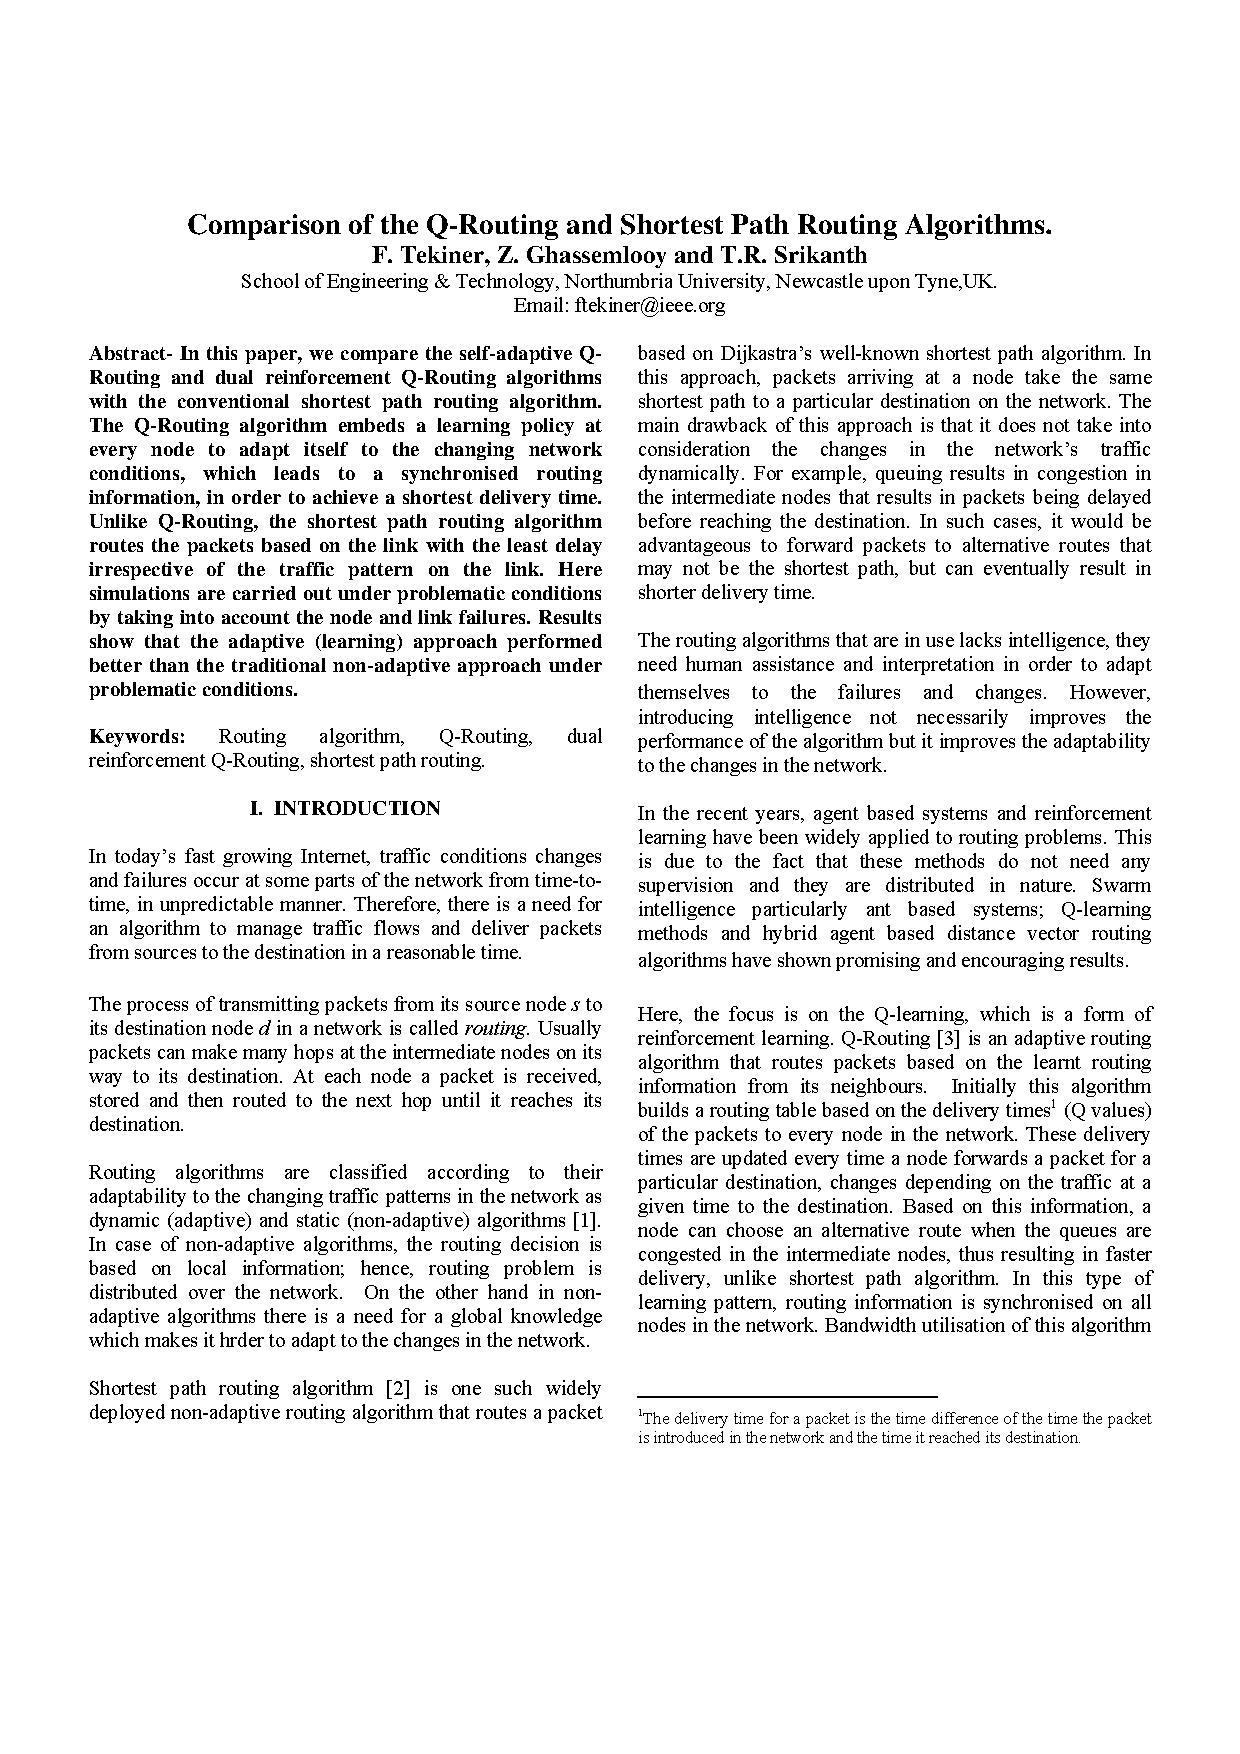
\includegraphics[width=17.5cm]{pic/translate/page-1.pdf}}

\end{figure}
% \begin{figure}[H]
%     \centering
%     \makebox[0pt]{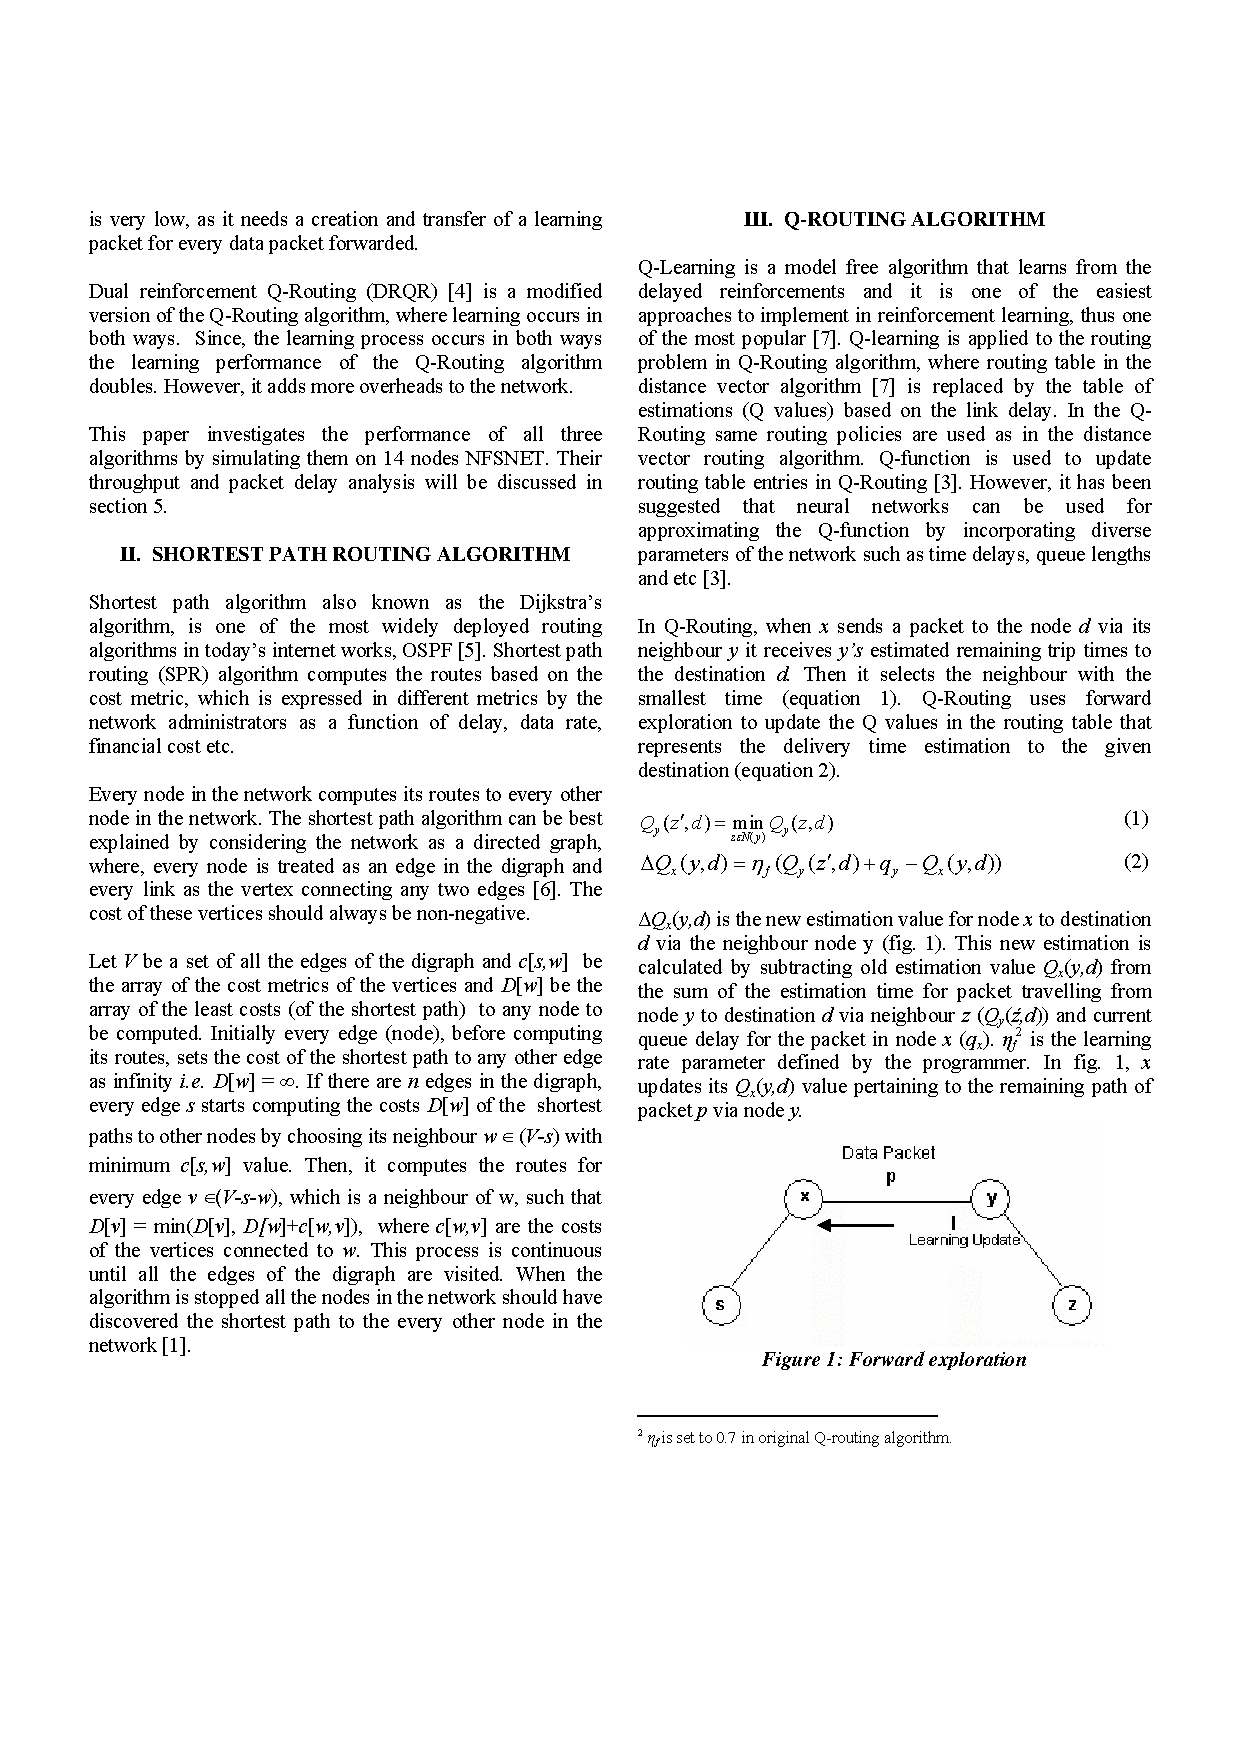
\includegraphics[width=17.5cm]{pic/translate/page-2.pdf}}

% \end{figure}
% \begin{figure}[H]
%     \centering
%     \makebox[0pt]{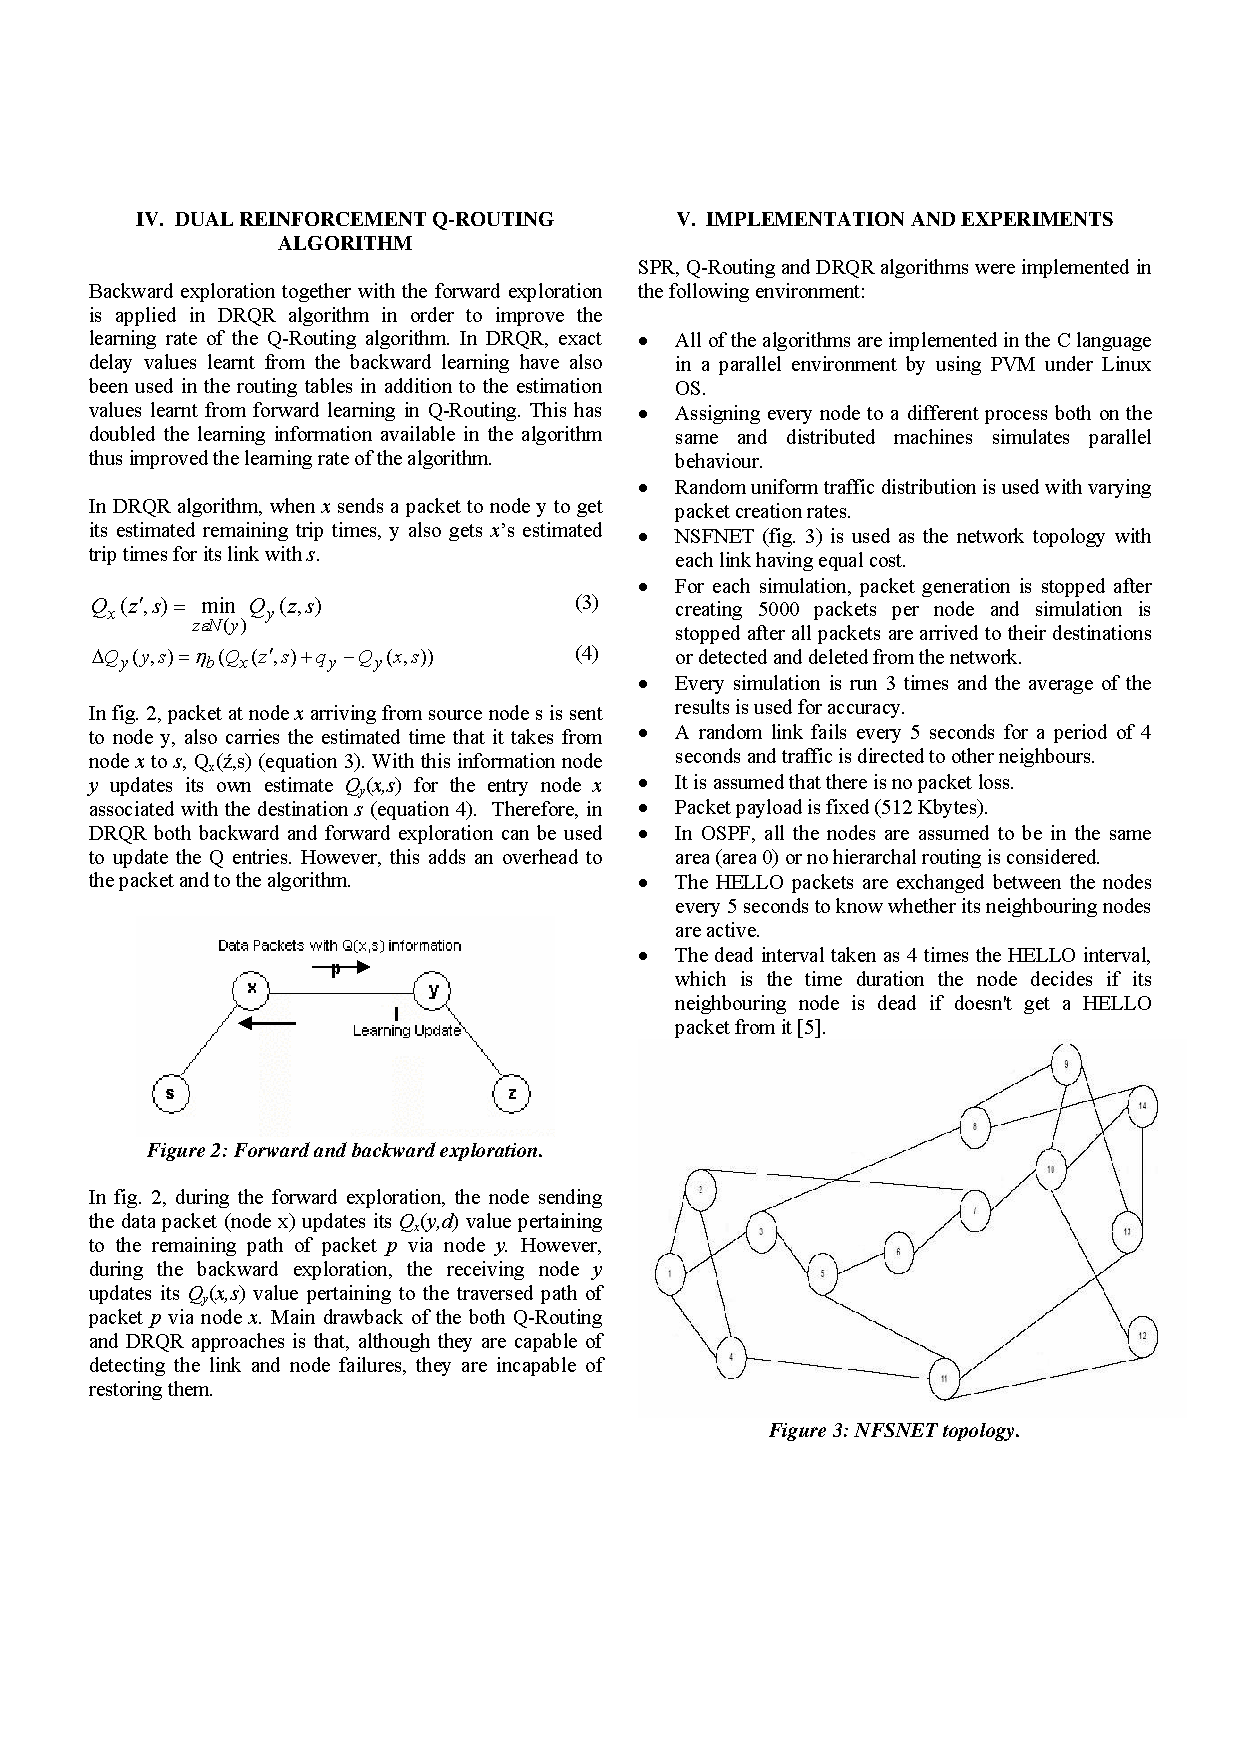
\includegraphics[width=17.5cm]{pic/translate/page-3.pdf}}

% \end{figure}
% \begin{figure}[H]
%     \centering
%     \makebox[0pt]{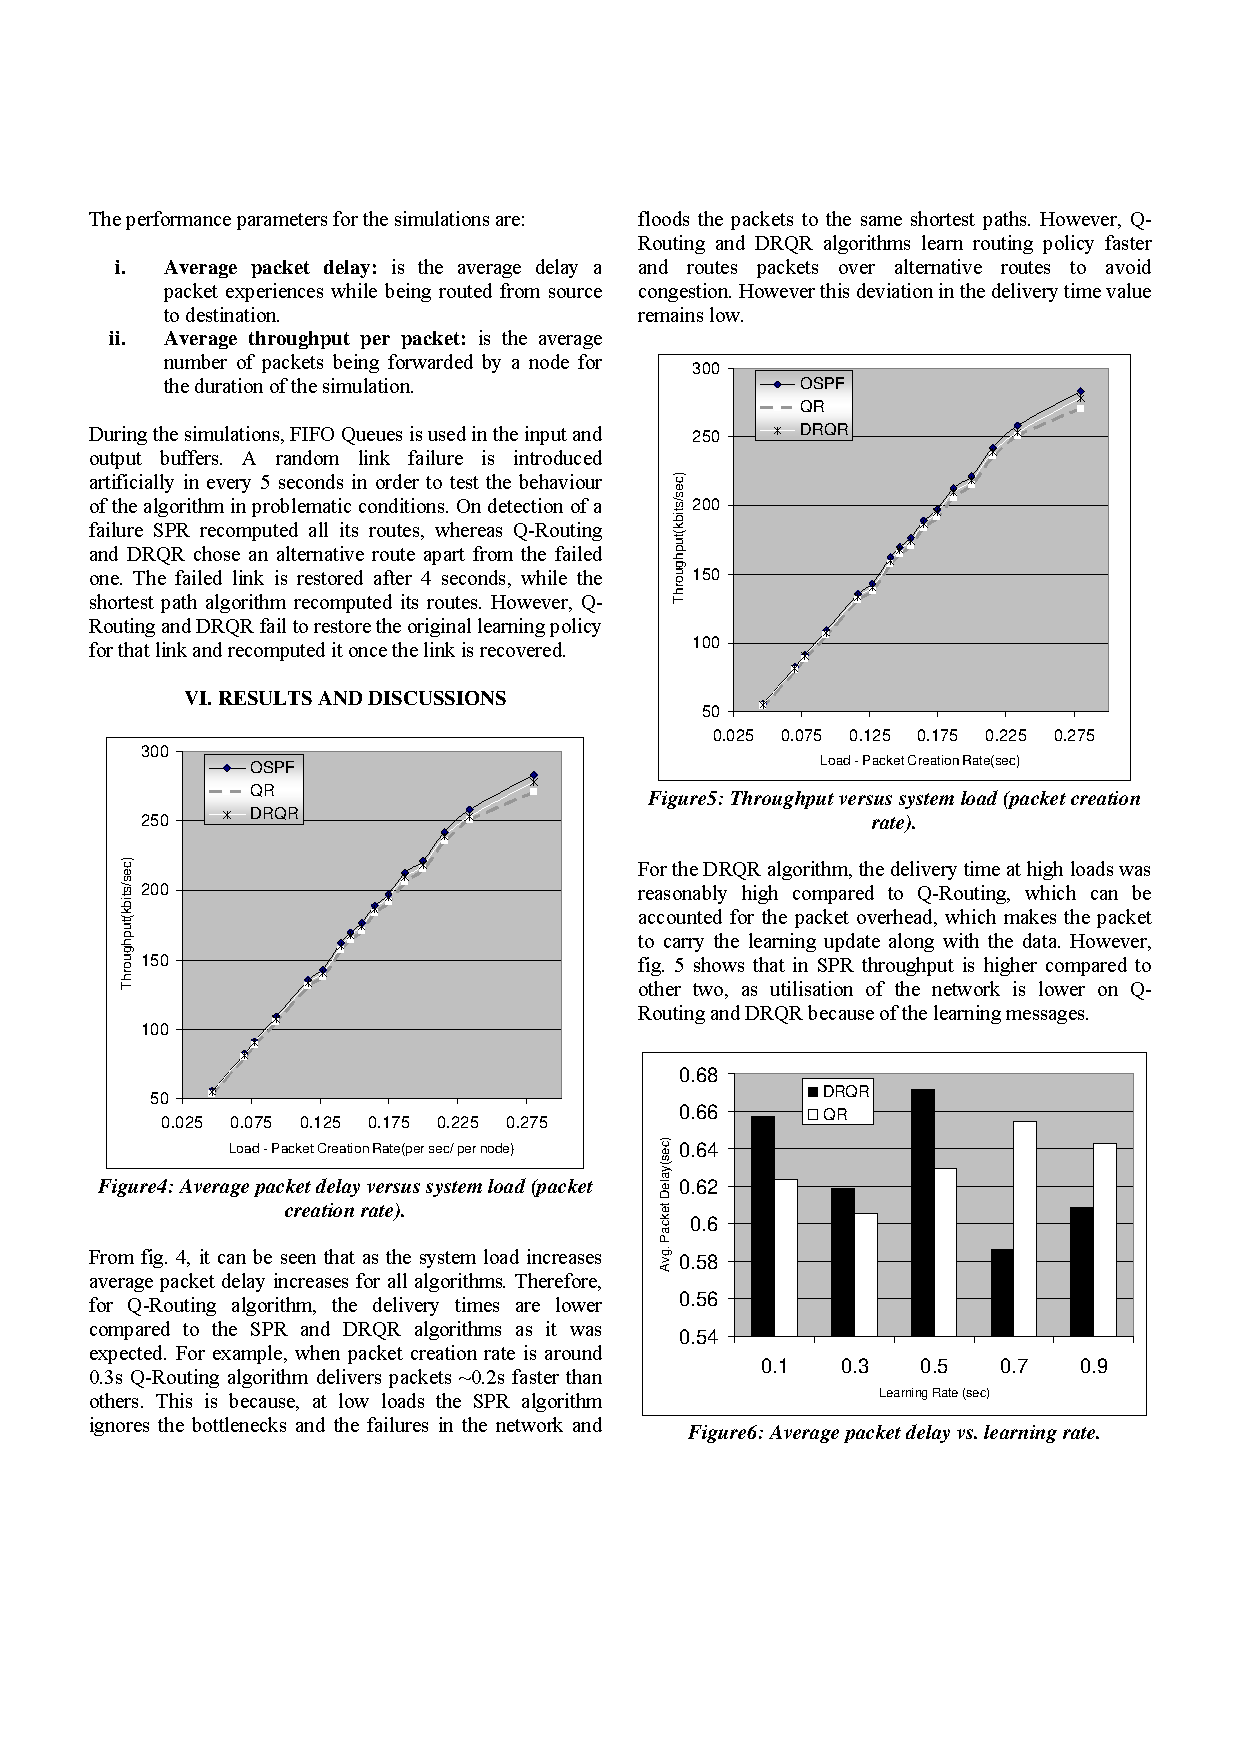
\includegraphics[width=17.5cm]{pic/translate/page-4.pdf}}

% \end{figure}
% \begin{figure}[H]
%     \centering
%     \makebox[0pt]{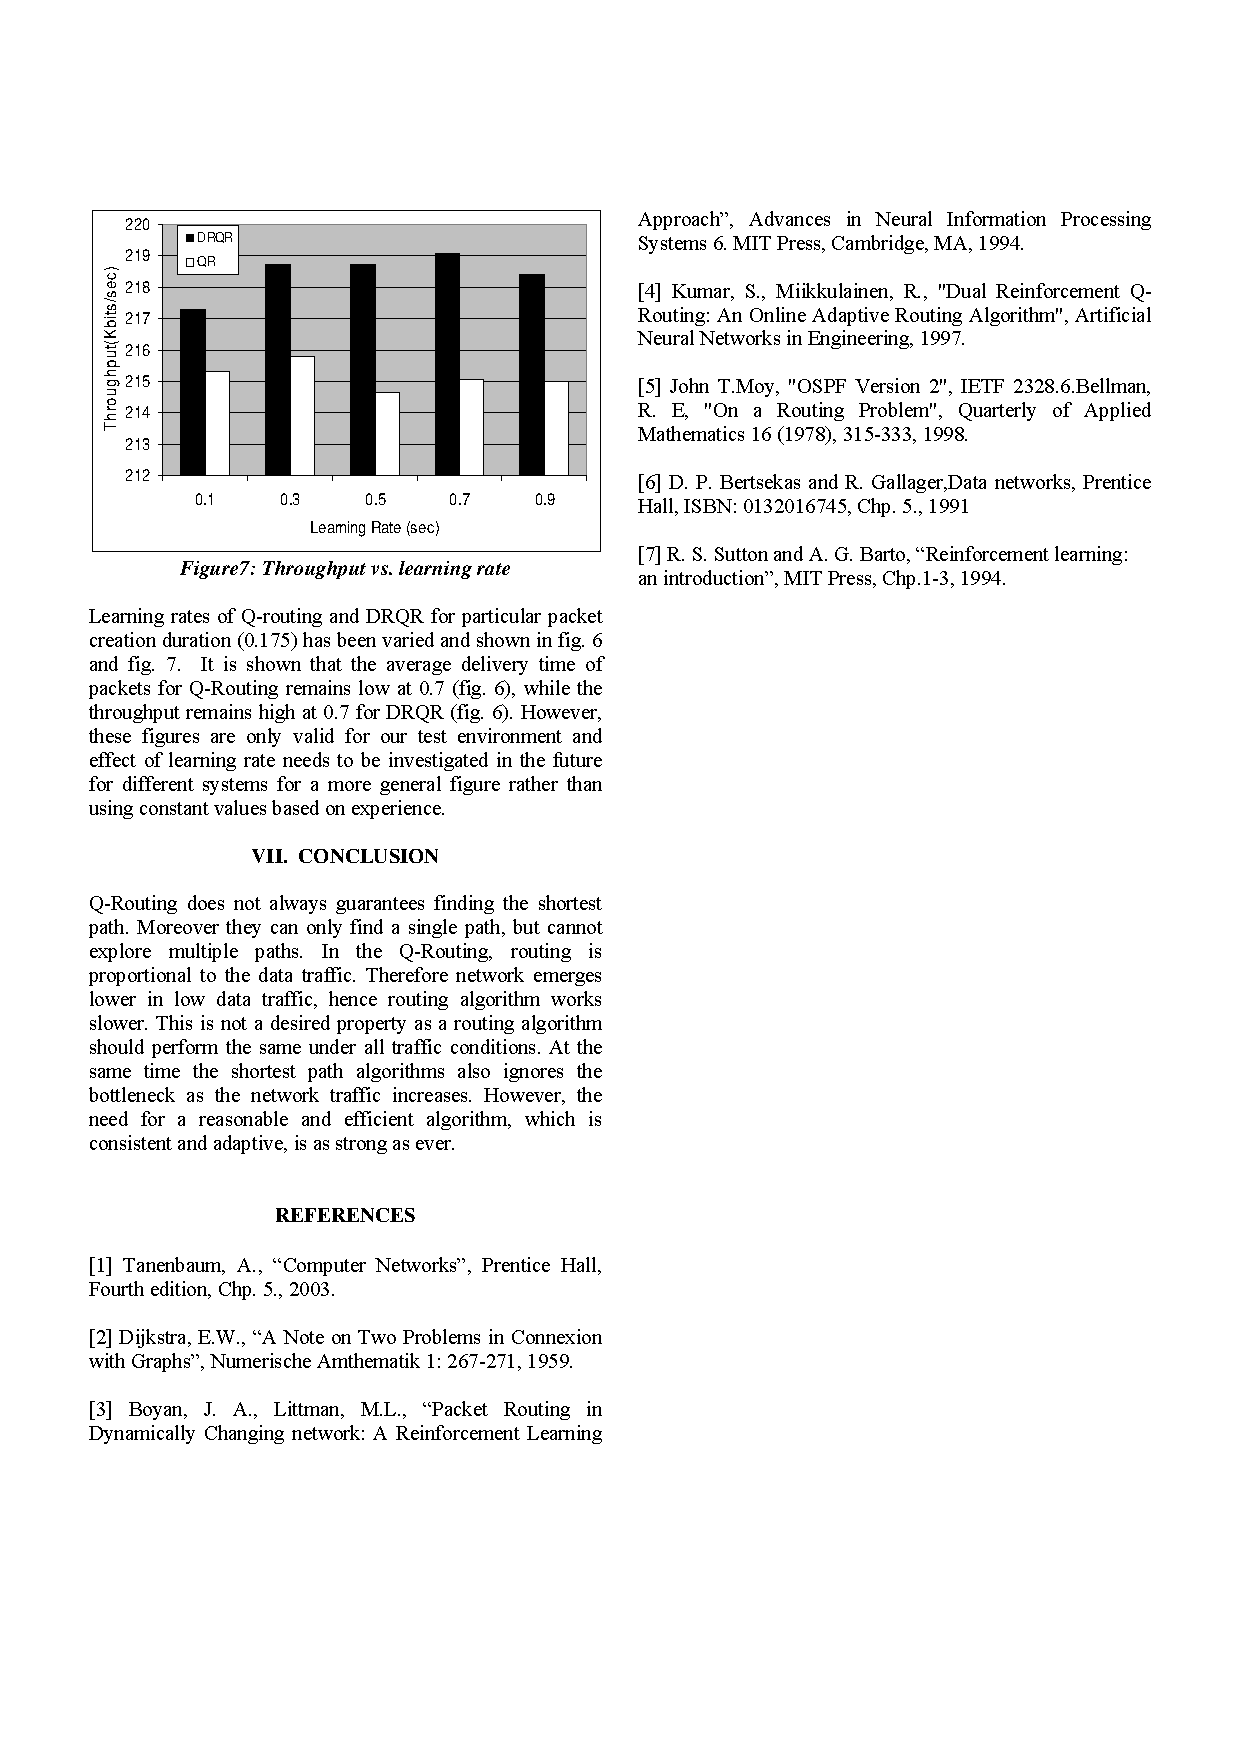
\includegraphics[width=17.5cm]{pic/translate/page-5.pdf}}

% \end{figure}
\end{document}
\documentclass{standalone}
% preamble: usepackage, etc.
\begin{document}
\thesistranslationchinese
\section{11测试}
\subsection{第1章}
\subsection{第二章}

\end{document}

\end{document}
